% Options for packages loaded elsewhere
\PassOptionsToPackage{unicode}{hyperref}
\PassOptionsToPackage{hyphens}{url}
%
\documentclass[
  doc,floatsintext]{apa6}
\usepackage{amsmath,amssymb}
\usepackage{iftex}
\ifPDFTeX
  \usepackage[T1]{fontenc}
  \usepackage[utf8]{inputenc}
  \usepackage{textcomp} % provide euro and other symbols
\else % if luatex or xetex
  \usepackage{unicode-math} % this also loads fontspec
  \defaultfontfeatures{Scale=MatchLowercase}
  \defaultfontfeatures[\rmfamily]{Ligatures=TeX,Scale=1}
\fi
\usepackage{lmodern}
\ifPDFTeX\else
  % xetex/luatex font selection
\fi
% Use upquote if available, for straight quotes in verbatim environments
\IfFileExists{upquote.sty}{\usepackage{upquote}}{}
\IfFileExists{microtype.sty}{% use microtype if available
  \usepackage[]{microtype}
  \UseMicrotypeSet[protrusion]{basicmath} % disable protrusion for tt fonts
}{}
\makeatletter
\@ifundefined{KOMAClassName}{% if non-KOMA class
  \IfFileExists{parskip.sty}{%
    \usepackage{parskip}
  }{% else
    \setlength{\parindent}{0pt}
    \setlength{\parskip}{6pt plus 2pt minus 1pt}}
}{% if KOMA class
  \KOMAoptions{parskip=half}}
\makeatother
\usepackage{xcolor}
\usepackage{graphicx}
\makeatletter
\def\maxwidth{\ifdim\Gin@nat@width>\linewidth\linewidth\else\Gin@nat@width\fi}
\def\maxheight{\ifdim\Gin@nat@height>\textheight\textheight\else\Gin@nat@height\fi}
\makeatother
% Scale images if necessary, so that they will not overflow the page
% margins by default, and it is still possible to overwrite the defaults
% using explicit options in \includegraphics[width, height, ...]{}
\setkeys{Gin}{width=\maxwidth,height=\maxheight,keepaspectratio}
% Set default figure placement to htbp
\makeatletter
\def\fps@figure{htbp}
\makeatother
\setlength{\emergencystretch}{3em} % prevent overfull lines
\providecommand{\tightlist}{%
  \setlength{\itemsep}{0pt}\setlength{\parskip}{0pt}}
\setcounter{secnumdepth}{-\maxdimen} % remove section numbering
% Make \paragraph and \subparagraph free-standing
\ifx\paragraph\undefined\else
  \let\oldparagraph\paragraph
  \renewcommand{\paragraph}[1]{\oldparagraph{#1}\mbox{}}
\fi
\ifx\subparagraph\undefined\else
  \let\oldsubparagraph\subparagraph
  \renewcommand{\subparagraph}[1]{\oldsubparagraph{#1}\mbox{}}
\fi
% definitions for citeproc citations
\NewDocumentCommand\citeproctext{}{}
\NewDocumentCommand\citeproc{mm}{%
  \begingroup\def\citeproctext{#2}\cite{#1}\endgroup}
\makeatletter
 % allow citations to break across lines
 \let\@cite@ofmt\@firstofone
 % avoid brackets around text for \cite:
 \def\@biblabel#1{}
 \def\@cite#1#2{{#1\if@tempswa , #2\fi}}
\makeatother
\newlength{\cslhangindent}
\setlength{\cslhangindent}{1.5em}
\newlength{\csllabelwidth}
\setlength{\csllabelwidth}{3em}
\newenvironment{CSLReferences}[2] % #1 hanging-indent, #2 entry-spacing
 {\begin{list}{}{%
  \setlength{\itemindent}{0pt}
  \setlength{\leftmargin}{0pt}
  \setlength{\parsep}{0pt}
  % turn on hanging indent if param 1 is 1
  \ifodd #1
   \setlength{\leftmargin}{\cslhangindent}
   \setlength{\itemindent}{-1\cslhangindent}
  \fi
  % set entry spacing
  \setlength{\itemsep}{#2\baselineskip}}}
 {\end{list}}
\usepackage{calc}
\newcommand{\CSLBlock}[1]{\hfill\break\parbox[t]{\linewidth}{\strut\ignorespaces#1\strut}}
\newcommand{\CSLLeftMargin}[1]{\parbox[t]{\csllabelwidth}{\strut#1\strut}}
\newcommand{\CSLRightInline}[1]{\parbox[t]{\linewidth - \csllabelwidth}{\strut#1\strut}}
\newcommand{\CSLIndent}[1]{\hspace{\cslhangindent}#1}
\ifLuaTeX
\usepackage[bidi=basic]{babel}
\else
\usepackage[bidi=default]{babel}
\fi
\babelprovide[main,import]{english}
% get rid of language-specific shorthands (see #6817):
\let\LanguageShortHands\languageshorthands
\def\languageshorthands#1{}
% Manuscript styling
\usepackage{upgreek}
\captionsetup{font=singlespacing,justification=justified}

% Table formatting
\usepackage{longtable}
\usepackage{lscape}
% \usepackage[counterclockwise]{rotating}   % Landscape page setup for large tables
\usepackage{multirow}		% Table styling
\usepackage{tabularx}		% Control Column width
\usepackage[flushleft]{threeparttable}	% Allows for three part tables with a specified notes section
\usepackage{threeparttablex}            % Lets threeparttable work with longtable

% Create new environments so endfloat can handle them
% \newenvironment{ltable}
%   {\begin{landscape}\centering\begin{threeparttable}}
%   {\end{threeparttable}\end{landscape}}
\newenvironment{lltable}{\begin{landscape}\centering\begin{ThreePartTable}}{\end{ThreePartTable}\end{landscape}}

% Enables adjusting longtable caption width to table width
% Solution found at http://golatex.de/longtable-mit-caption-so-breit-wie-die-tabelle-t15767.html
\makeatletter
\newcommand\LastLTentrywidth{1em}
\newlength\longtablewidth
\setlength{\longtablewidth}{1in}
\newcommand{\getlongtablewidth}{\begingroup \ifcsname LT@\roman{LT@tables}\endcsname \global\longtablewidth=0pt \renewcommand{\LT@entry}[2]{\global\advance\longtablewidth by ##2\relax\gdef\LastLTentrywidth{##2}}\@nameuse{LT@\roman{LT@tables}} \fi \endgroup}

% \setlength{\parindent}{0.5in}
% \setlength{\parskip}{0pt plus 0pt minus 0pt}

% Overwrite redefinition of paragraph and subparagraph by the default LaTeX template
% See https://github.com/crsh/papaja/issues/292
\makeatletter
\renewcommand{\paragraph}{\@startsection{paragraph}{4}{\parindent}%
  {0\baselineskip \@plus 0.2ex \@minus 0.2ex}%
  {-1em}%
  {\normalfont\normalsize\bfseries\itshape\typesectitle}}

\renewcommand{\subparagraph}[1]{\@startsection{subparagraph}{5}{1em}%
  {0\baselineskip \@plus 0.2ex \@minus 0.2ex}%
  {-\z@\relax}%
  {\normalfont\normalsize\itshape\hspace{\parindent}{#1}\textit{\addperi}}{\relax}}
\makeatother

\makeatletter
\usepackage{etoolbox}
\patchcmd{\maketitle}
  {\section{\normalfont\normalsize\abstractname}}
  {\section*{\normalfont\normalsize\abstractname}}
  {}{\typeout{Failed to patch abstract.}}
\patchcmd{\maketitle}
  {\section{\protect\normalfont{\@title}}}
  {\section*{\protect\normalfont{\@title}}}
  {}{\typeout{Failed to patch title.}}
\makeatother

\usepackage{xpatch}
\makeatletter
\xapptocmd\appendix
  {\xapptocmd\section
    {\addcontentsline{toc}{section}{\appendixname\ifoneappendix\else~\theappendix\fi\\: #1}}
    {}{\InnerPatchFailed}%
  }
{}{\PatchFailed}
\usepackage{csquotes}
\usepackage{placeins} 

\ifLuaTeX
  \usepackage{selnolig}  % disable illegal ligatures
\fi
\usepackage{bookmark}
\IfFileExists{xurl.sty}{\usepackage{xurl}}{} % add URL line breaks if available
\urlstyle{same}
\hypersetup{
  pdftitle={Who mistrust basic science?},
  pdflang={en-EN},
  hidelinks,
  pdfcreator={LaTeX via pandoc}}

\title{Who mistrust basic science?}
\author{\phantom{0}}
\date{}


\shorttitle{Who mistrust basic science?}

\affiliation{\vspace{0.5cm}\textsuperscript{} }

\abstract{%
XX
}



\begin{document}
\maketitle

\section{Introduction}\label{introduction}

There is increasingly more talk of defiance towards science and towards experts more generally. In every population, many people only trust science `some of the time', and a sizable minority doesn't trust it.

This appears difficult to reconcile with the fact that, in many countries, most people receive at least a basic science education, that science education (along with education more generally) is increasing, and that science education seems to be the main driver of trust in science.

But how deep is distrust of science? Do people reject science wholesale, or is it more driven by attitudes towards specific contents, maybe in particular those seen as being politicized, or as going against deeply held beliefs, or behaviors they want to engage in? {[}previous work suggests that issue-specific claims provoke more negative attitudes{]}

Here, we look at whether people in the US, across different levels of trust in science (including a sample with anti-vaccine attitudes), accept basic scientific facts.

{[}We can draw some inspiration from the ``Westwood et al 2021 Current research overstates American support for political violence'' paper: we want to put in perspective the current rise (? discourse around?) in mistrust towards science{]}

\subsection{Levels of trust in science}\label{levels-of-trust-in-science}

\subsection{Why do people distrust science?}\label{why-do-people-distrust-science}

{[}here? We know from the many studies on the gateway belief model that people don't always accept the scientific consensus (indeed, the effect sizes are usually not massive){]}

\subsection{How much science do people know?}\label{how-much-science-do-people-know}

This is a crucial point: if there are questions with specific scientific answers that just about everyone already knows, then in a sense our point is already proven\ldots{} so the first thing to do would be to look at data on knowledge of science, and see what the highest rates of correct answer is, to see how much room for improvement there is.

``The dominant approach to conceptualizing and measuring science literacy in population surveys has arisen out of work by Jon D. Miller and Kenneth Prewitt in the United States (see Miller, 1983, 1998, 2004) alongside collabora- tors in Great Britain (see Durant et al., 1989). Underlying these efforts appears to have been widespread concern among policy makers and the scientific com- munity that nonscientists were becoming skeptical about the benefits of sci- ence and that such skepticism might result in cuts to science funding that would harm the scientific progress that many argue underpins both American and European economic development (Bauer et al., 2007). The results of the U.S. portion of this work have formed the core of a chapter of a biennial report called Science and Engineering Indicators (hereafter, Indicators) that the National Science Board provides to Congress and the Executive Branch. Scholars have also used the raw data collected for Indicators (which is made publicly available) for peer-reviewed research (e.g., Gauchat, 2012; Losh, 2010), and other countries have used many of the Indicators' questions for their own national surveys (e.g., Bauer et al., 2012a; National Science Board, 2016).''

\section{Overview of experiments}\label{overview-of-experiments}

The goal is to see to which extent people do not accept basic science.

\section{Experiment 1}\label{experiment-1}

The main goal of experiment one was to test whether people would accept the scientific consensus on basic knowledge questions. Additionally, we wanted to know if both science knowledge and acceptance of the scientific consensus are associated with trust in science and conspiracy thinking. We had the following research questions:

\textbf{RQ1: What is the average science knowledge score (1)?}

\textbf{RQ2: What is the average acceptance of the scientific consensus (2)?}

\textbf{RQ3: What is the relationship between trust in science and, respectively, (1) and (2)?}

\textbf{RQ4: What is the relationship between conspiracy thinking and, respectively, (1) and (2)?}

\subsection{Methods}\label{methods}

\subsubsection{Participants}\label{participants}

We recruited 200 participants from the US via prolific. 6 participants failed our attention check, resulting in a final sample of 194 participants (98 female, 96 male; \(age_\text{mean}\): 41.71, \(age_\text{sd}\): 13.07, \(age_\text{median}\): 39). Since we did not have any prior assumptions on effect sizes, we did not do a power analysis.

\subsubsection{Procedure}\label{procedure}

After providing their consent to participate in the study, participants were given an attention check ``While watching the television, have you ever had a fatal heart attack?'' {[}1-6; 1 = Never, 6 = Often{]}. All participants who did not answer ``1 = Never'' were excluded. Participants then read the following instructions:``We will ask you 11 questions about science. After each question, we will provide you with the scientifically consensual answer and ask whether you accept it.'' Next, participants answered a set of 10 basic science questions, which were randomly selected from a pool of 11 questions, in random order. After each question, participants were presented with an answer reflecting the scientific consensus. Participants were asked to choose whether they accept the answer or not, before proceeding to the next question. Figure \ref{fig:stimulus-example} displays the survey for an example science question. Finally, participants answered questions on conspiracy thinking and trust in science.



\begin{figure}

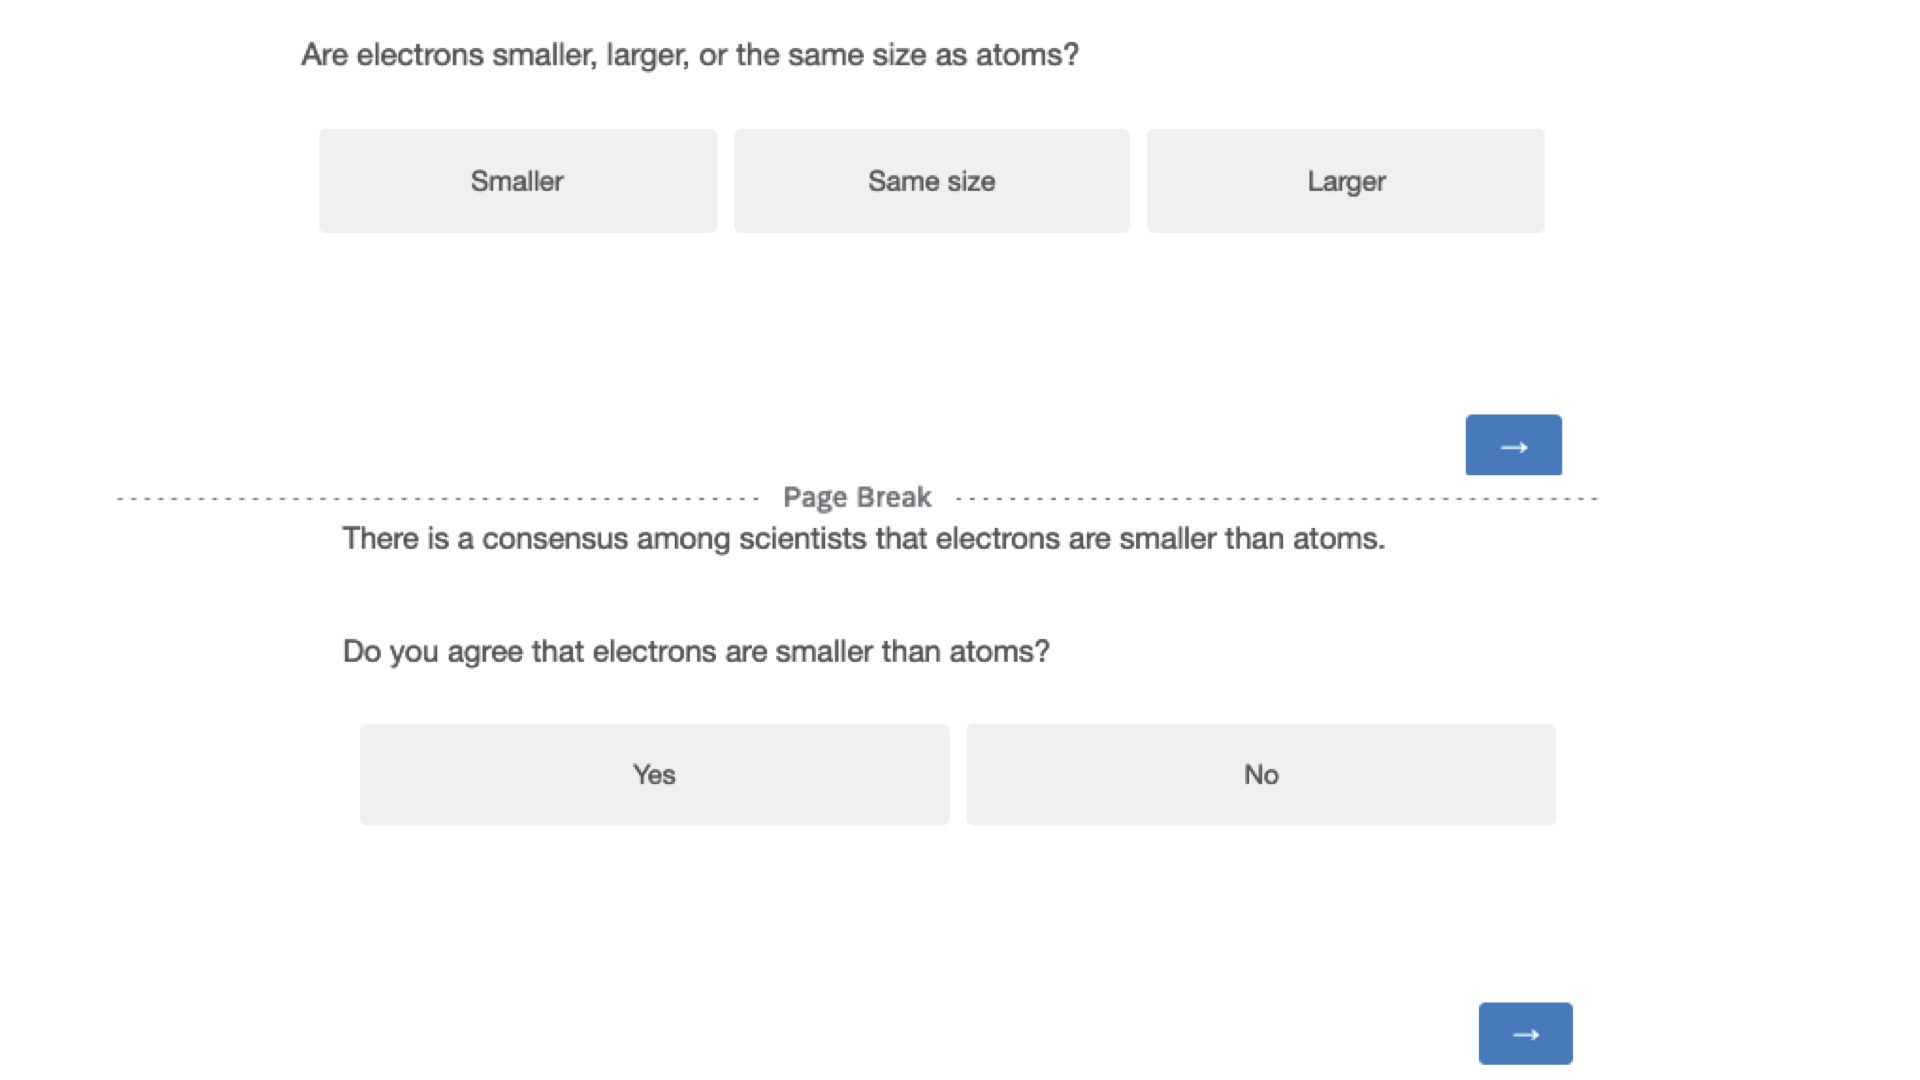
\includegraphics[width=1\linewidth]{./figures/study1_question_example} \hfill{}

\caption{Example of a science question, the scientific consensus and the corresponding acceptance question.}\label{fig:stimulus-example}
\end{figure}

\subsubsection{Materials}\label{materials}

\paragraph{Science knowledge and acceptance}\label{science-knowledge-and-acceptance}

Table \ref{tab:knowledge} shows all questions, their scientifically consensual answer, and their source. All but two questions were selected from existing science knowledge questionnaires. We tried to select non-political questions.

\begingroup\fontsize{8}{10}\selectfont

\begin{longtable}[t]{>{\raggedleft\arraybackslash}p{1em}>{\raggedright\arraybackslash}p{10em}>{\raggedright\arraybackslash}p{10em}>{\raggedright\arraybackslash}p{23em}}
\caption{\label{tab:knowledge}Science knowledge items}\\
\toprule
id & Question & Scientific consensus (Study 1) & Explanation (Study 2 \& 3)\\
\midrule
1 & Do antibiotics kill viruses as well as bacteria? & There is a consensus among scientists that antibiotics kill bacteria, but not viruses. & Antibiotics specifically target and kill bacteria, not viruses. Scientists know this thanks to extensive laboratory experiments and clinical trials where antibiotics have been observed to be effective against bacterial infections but not viral ones. Scientists have also studied how antibiotics work, which typically involve disrupting bacterial cell processes like cell wall synthesis or protein production, which are absent in viruses.

Here are some resources confirming that antibiotics only kill bacteria: 
American Chemical Society
Queensland Government 
Wikipedia\\
2 & Are electrons smaller, larger, or the same size as atoms ? & There is a consensus among scientists that electrons are smaller than atoms. & Electrons are much smaller than atoms. Scientists know this thanks to experiments in particle physics, such as electron scattering experiments. They are also able to measure the electron charge and mass. Additionally, atomic theory and quantum mechanics provide a theoretical framework explaining the structure of atoms, where electrons orbit the nucleus in distinct energy levels.

Here are some resources confirming that electrons are smaller than atoms:
Science Focus 
Britannica 
Wikipedia\\
3 & Have the continents on Earth been moving for millions of years or have they always been where they are now? & There is a consensus among scientists that the continents on Earth have been moving for millions of years due to plate tectonics. & The continents on Earth have been moving for millions of years due to plate tectonics. Scientists have gathered evidence from various sources, including fossil records, geological formations, and the magnetic properties of rocks. The theory of plate tectonics explains how the Earth's lithosphere is divided into large, rigid plates that move over the semi-fluid asthenosphere, leading to phenomena like continental drift, earthquakes, and volcanic activity.

Here are some resources confirming that continents on Earth have been moving for millions years:
Britannica 
Live Science 
National Geographic\\
4 & What decides whether a baby is a boy or a girl ? Is it the father’s genes, the mother’s genes, or both? & There is a consensus among scientists that it is the genes in the father's sperm which are decisive on whether a baby is a boy or a girl. & Chromosomes are structures found in the nucleus of cells that carry long pieces of DNA. Two of the chromosomes (the X and the Y chromosome) are called sex chromosomes. In most cases, females have two X chromosomes, while males have one X and one Y chromosome. At conception, the mother transmits an X chromosome, and the father may contribute an X or a Y. The chromosome from the father therefore determines if the baby is female (if the father transmits an X) or male (if the father transmits a Y). In most cases, children are born a male or female according to their chromosomes. However, some children may be born with genitalia that do not match their chromosomes.

Here are some resources confirming that it is the father's genes that decide the sex of a baby: 
National Library of Medicine 
Nature 
Wikipedia\\
5 & Do lasers work by focusing sound waves? & There is a consensus among scientists that lasers do not work by focusing sound waves. & Lasers produce a narrow beam of light in which all of the particles of light have very similar wavelengths. The laser’s lightwaves travel together with their peaks all lined up, in phase. This is why laser beams are very narrow, very bright, and can be focused into a very tiny spot. Because laser light stays focused and does not spread out much (like a flashlight would), laser beams can travel very long distances.

Here are some resources confirming that lasers do not work by focusing sound waves: 
NASA 
Lawrence Livermore National Library
Wikipedia\\
\addlinespace
6 & How long does it take for Earth to go around the sun: one day, one month, or one year ? & There is a consensus among scientists that it takes one year for Earth to go around the sun. & Earth takes approximately one year to orbit the sun. This knowledge is based on astronomical observations and measurements of celestial motion. Early astronomers tracked the movement of the Earth relative to the stars and planets, leading to the development of models that accurately predict the Earth's orbital period around the sun.

Here are some resources confirming that Earth goes around the sun in one year: 
NASA
National Geographic 
Wikipedia\\
7 & Are diamonds made of carbon ? & There is a consensus among scientists that diamonds are made of carbon. & Diamonds are made of only one element, carbon. Carbon is the same element that makes coal or graphite used for pencils. Why are diamonds transparent and hard while coal and graphite are opaque and soft? It all comes down to the placement of their atoms. In diamonds, each carbon atom is bonded to 4 other carbon atoms, while in graphite, each atom is only bonded to 3 other carbon atoms. The bonds in diamonds are held in such a tight structure that all light passes around them, which is why diamonds look transparent. In coal and graphite, light gets trapped between the atoms, which is why they look dark and opaque. Why do carbon atoms bond differently in diamonds? At very high pressures and temperatures, the carbon atoms are squeezed so much that they start touching more atoms. When the pressure is about 50,000 times the pressure at the surface of the Earth and the temperature is about 1600°C, the carbon atoms bond with 4 other atoms and result in diamonds.

Here are some resources confirming that diamonds are made of carbon: 
Arizona State University 
University of Bristol 
Wikipedia\\
8 & Which travels faster : light or sound? & There is a consensus among scientists that light travels faster than sound. & Light travels faster than sound. This conclusion arises from numerous experiments and observations in physics. You can also experience this for yourself during a thunderstorm. Unless the lighting is right above you, you will first see the lighting, then hear the thunder some time after (you can even tell how far the lighting struck by counting how many seconds it takes for the thunder to reach you). More precisely, the speed of light has been measured accurately using techniques such as the Michelson–Morley experiment. Similarly, the speed of sound has been measured through experiments involving the propagation of sound waves through various materials.

Here are some resources confirming that light travers faster than sound: 
NASA 
Wikipedia : Speed of light 
Wikipedia: Speed of sound\\
9 & Is common table salt made of calcium carbonate? & There is a consensus among scientists that common table salt is not made of calcium carbonate; it is made of sodium chloride. & Common table salt, or sodium chloride (NaCl), is not made of calcium carbonate. Scientists can use a variety of tests to understand what matter is made of. The most used test for sodium chloride is the chemical reaction with silver nitrate. The presence of sodium chloride yields a white precipitate upon drops of a silver nitrate solution. Calcium carbonate, by contrast, is the substance that makes up, for instance, chalk.

Here are some resources confirming that common table salt is not made of calcium carbonate: 
National Library of Medicine 
Chem Europe 
Wikipedia\\
10 & Is water made of molecules containing one oxygen and two hydrogen atoms? & There is a consensus among scientists that water is made of molecules containing one oxygen and two hydrogen atoms, and that its chemical formula is therefore H2O. & Water is made of molecules containing one oxygen atom and two hydrogen atoms, chemically represented as H2O. We know this for instance because if you set hydrogen on fire in a container with oxygen, water will form on the sides of the container. More recent techniques such as spectroscopy and X-ray crystallography have allowed scientists to more directly see the composition and structure of water molecules, confirming the presence of two hydrogen atoms bonded to one oxygen atom.

Here are some resources confirming that water is made of molecules containing one oxygen and two hydrogen atoms:
National Library of Medicine 
Wikipedia: Chemical structure 
Wikipedia: Water\\
\addlinespace
11 & Where do trees mainly draw the materials with which they create their mass? & There is a consensus among scientists that carbon drawn from the air during photosynthesis makes up most of the materials that trees use to build new leaves, stems, and roots. & \\
\bottomrule
\end{longtable}
\endgroup{}

\paragraph{Conspiracy scales}\label{conspiracy-scales}

To measure conspiracy thinking, we selected 10 science/health related conspiracy theories from the Belief in Conspiracy Theory Inventory (BCTI) by Pennycook, Binnendyk, and Rand (2022) (Table \ref{tab:conspiracy}).

\begingroup\fontsize{8}{10}\selectfont

\begin{longtable}[t]{>{}r>{\raggedright\arraybackslash}p{40em}}
\caption{\label{tab:conspiracy}Conspiracy items}\\
\toprule
1 & The Apollo moon landings never happened and were staged in a Hollywood film studio.\\
2 & A cure for cancer was discovered years ago, but this has been suppressed by the pharmaceutical industry and the U.S. Food and Drug Administration (FDA).\\
3 & The spread of certain viruses and/or diseases is the result of the deliberate, concealed efforts of vested interests.\\
4 & The claim that the climate is changing due to emissions from fossil fuels is a hoax perpetrated by corrupt scientists who want to spend more taxpayer money on climate research.\\
5 & The Earth is flat (not spherical) and this fact has been covered up by scientists and vested interests.\\
\addlinespace
6 & There is a causal link between vaccination and autism that has been covered up by the pharmaceutical industry.\\
7 & In the 1950s and 1960s more than 100 million Americans received a polio vaccine contaminated with a potentially cancer-causing virus.\\
8 & Proof of alien contact is being concealed from the public.\\
9 & Hydroxychloroquine has been demonstrated to be a safe and effective treatment of COVID and this information is being suppressed.\\
10 & Dinosaurs never existed, evolution is not real, and scientists have been faking the fossil record.\\
\bottomrule
\end{longtable}
\endgroup{}

To cross-check our results with alternative measures, we also assessed the conspiracy mentality questionnaire (CMQ) by Bruder, Haffke, Neave, Nouripanah, and Imhoff (2013) and the Single Item Conspiracy Beliefs Scale (SICBS) by Lantian, Muller, Nurra, and Douglas (2016) (see Appendix \ref{exp1}).

\paragraph{Trust in science}\label{trust-in-science}

Our main item for measuring trust in science is selected from the Wellcome Global Monitor survey: ``In general, would you say that you trust science a lot, some, not much, or not at all? {[}1 = Not at all, 2 = Not much, 3 = Some, 4 = A lot{]}''

We also included two additional trust questions, one also from the Wellcome Global Monitor (WGM) survey (``How much do you trust scientists in this country? Do you trust them a lot, some, not much, or not at all? {[}1 = Not at all, 2 = Not much, 3 = Some, 4 = A lot{]}''), the other from the Pew research center (``How much confidence do you have in scientists to act in the best interests of the public? {[}1-5; 1 = No confidence at all, 5 = A great deal of confidence{]}''). We selected these items so that we could compare the ratings in our sample to global survey results. The WGM survey has been administered in over 140 countries and included over 140000 respondents. The Pew question has recently been used by a world-wide many labs study in 67 countries with 71417 respondents (Cologna et al., 2024).

\subsection{Results}\label{results}

Regarding RQ1 and RQ2, participants answered on average 74 \% (sd = 0.16) of the questions correctly, and accepted the scientific consensus on average for 93 \% (sd = 0.12) of the questions.

Fig. \ref{fig:exp1-conditional-acceptance} illustrates the relationship between knowledge and acceptance. In most cases (76.3 \%), participants readily accepted the scientific consensus after having given the wrong answer to a question. In very few cases (1.6 \%), participants who gave the correct response afterwards rejected the scientific consensus, thereby contradicting their own initial response. We believe this might have been due to inattention.



\begin{figure}
\centering
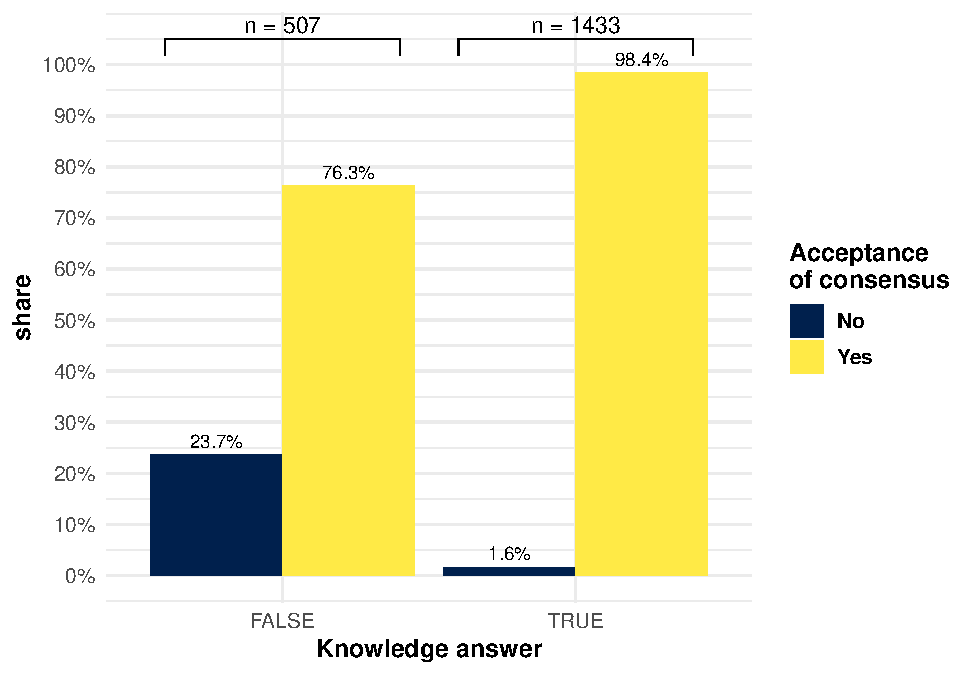
\includegraphics{output/figures/exp1-conditional-acceptance.pdf}
\caption{\label{fig:exp1-conditional-acceptance}Acceptance rates of scientific consensus, based on whether the initial response to the knowledge question was false or true.}
\end{figure}

For RQ3, we find a positive but small correlation between both science knowledge and trust in science (r = 0.29, p \textless{} .001), and acceptance of scientific consensus and trust in science (r = 0.27, p \textless{} .001). The more people are knowledgeable about science and the more they tend to accept the scientific consensus, the more they tend to trust science. These correlations are relatively weak, which might be partly due to ceiling effects: As illustrated in Fig. \ref{fig:exp1-plot}, (i) most people do trust science, and (ii) that is true even among people with low knowledge or acceptance rates.

For RQ4, we find a negative correlation of similar magnitude between conspiracy thinking and science knowledge (r = -0.38, p \textless{} .001), and conspiracy thinking and acceptance of scientific consensus (r = -0.33, p \textless{} .001).

In Appendix \ref{exp1}, we show that these associations are robust when using alternative measures of trust and conspiracy thinking. Appendix \ref{exp1} also includes more descriptive statistics, such as knowledge and acceptance by science questions.

Are trust in science and conspiracy thinking, respectively, associated with being more easily convinced of the scientific consensus? In our main analyses, we looked at correlations of acceptance across all observations. One possibility is that the associations between trust in science/conspiracy thinking and acceptance of scientific consensus are explained by science knowledge: People who give the right answer in the first place are more ready to accept the consensus, and trust in science/conspiracy thinking are mostly associated with this knowledge, but not with willingness to accept the consensus. To addressed this potential confound, in a non-preregistered analysis, we restricted our sample to cases where participants gave the wrong answer to the knowledge question. We than calculated the correlation between trust in science and average acceptance rate by participant. We find no statistically significant correlation of acceptance with neither conspiracy thinking (r = -0.14, p = 0.061), nor with trust in science (r = 0.06, p = 0.387).



\begin{figure}
\centering
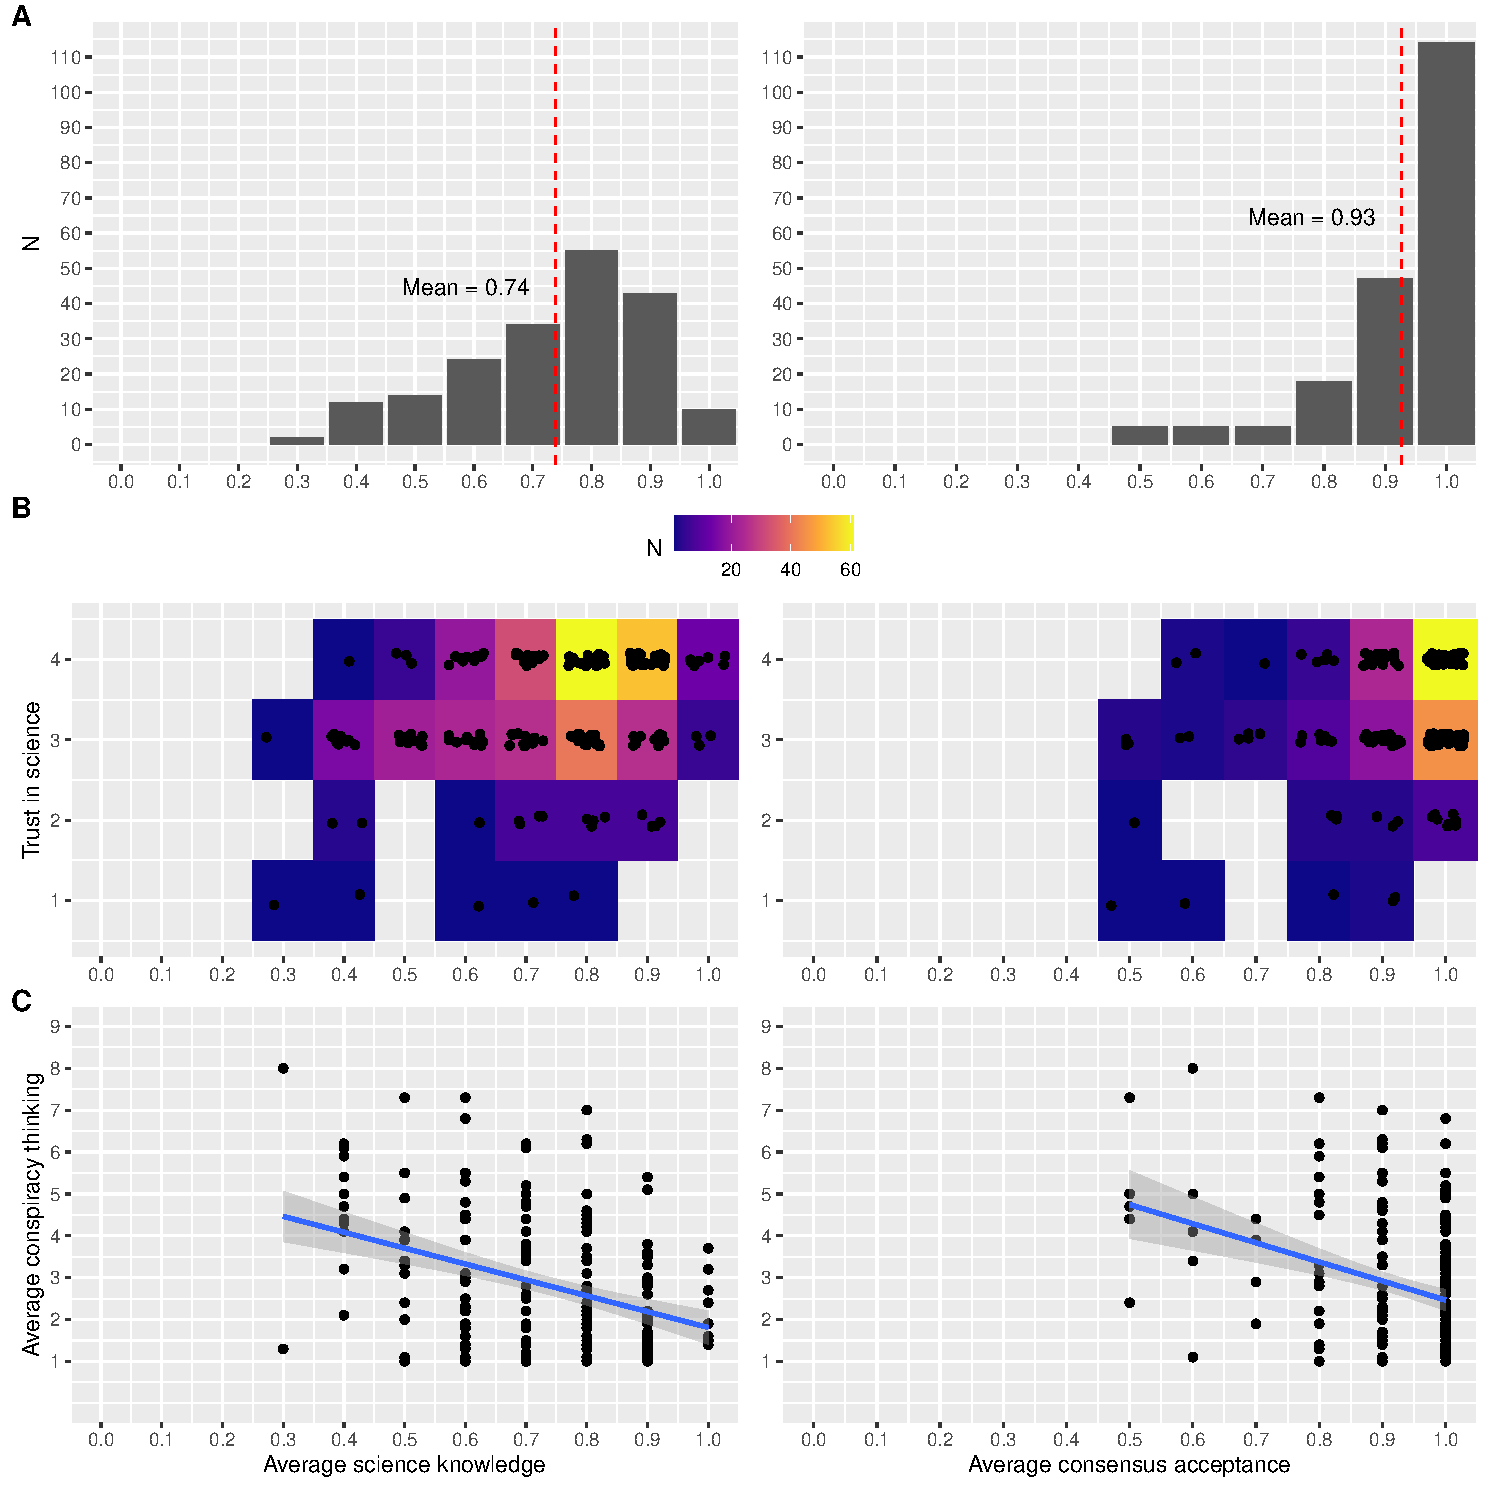
\includegraphics{output/figures/exp1-plot.pdf}
\caption{\label{fig:exp1-plot}\textbf{A} Shows the distribution of science knowledge (left) and acceptance of scientific consensus \textbf{B} Shows the relationship between trust in science and science knowledge/acceptance of scientific consensus \textbf{C} Shows the relationship between conspiracy thinking and science knowledge/acceptance of scientific consensus}
\end{figure}

\subsection{Discussion}\label{discussion}

These results suggest that most people accept the scientific consensus most of the time. Even when people do not know the correct answer to a science question, they tend to mostly accept the scientific consensus afterwards. Yet, in 23.7 \% of the cases, participants rejected the scientific consensus after having given the wrong answer, suggesting that simply stating the consensus is not sufficient to convince participants sometimes. In general, people with lower trust in science and who believe more in conspiracy theories tend to both know less about science and accept the scientific consensus less.

\section{Experiment 2}\label{experiment-2}

In experiment 1, we tested whether participants would accept the scientific consensus on basic science facts. In most instances they did, but not always. In experiment 2, we wanted to test whether this reluctance was because of participants not trusting us as a source of consensual science knowledge. To do so, we added an explanation and sources to each consensus statement, instead of only stating the consensus. To better understand reasons for consensus rejection, after having answered all questions, we asked participants an open-ended question to explain why they rejected the consensus, for each question on which they did so. We also excluded the where do trees their materials from, as this question clearly seemed to be an outlier where most participants would get the answer wrong (see Appendix \ref{exp1}).

Based on experiment 1, we formulated the following hypotheses:

\textbf{H1a: Higher trust in science is associated with more science knowledge?}

\textbf{H1b: Higher trust in science is associated with more acceptance of the scientific consensus, for participants who did not already know it?}

\textbf{H2a: Higher conspiracy thinking is associated with less science knowledge?}

\textbf{H2b: Higher conspiracy thinking is associated with less acceptance of the scientific consensus, for participants who did not already know it?}

We had the following research questions:

\textbf{RQ1: What is the average science knowledge score?}

\textbf{RQ2: When a participant's answer does not match the consensus, how often do they change their mind and accept the consensus?}

\textbf{RQ3: What reasons do participants provide to justify their rejection of the scientific consensus?}

\subsection{Methods}\label{methods-1}

\subsubsection{Participants}\label{participants-1}

We recruited 201 participants from the US via prolific. 11 participants failed our attention check, resulting in a final sample of 190 participants (96 female, 94 male; \(age_\text{mean}\): 43.48, \(age_\text{sd}\): 12.25, \(age_\text{median}\): 42). Since we did not have any prior assumptions on effect sizes and our analyses were descriptive, we did not do a power analysis.

\subsubsection{Procedure}\label{procedure-1}

The procedure was the same as in experiment 1, with the difference that, instead of just stating the scientific consensus, participants were presented with a short explanation which we wrote, partly based on explanations generated by ChatGPT, and three links to authoritative sources supporting the answer (Fig. \ref{fig:exp2-stimulus-example}.



\begin{figure}

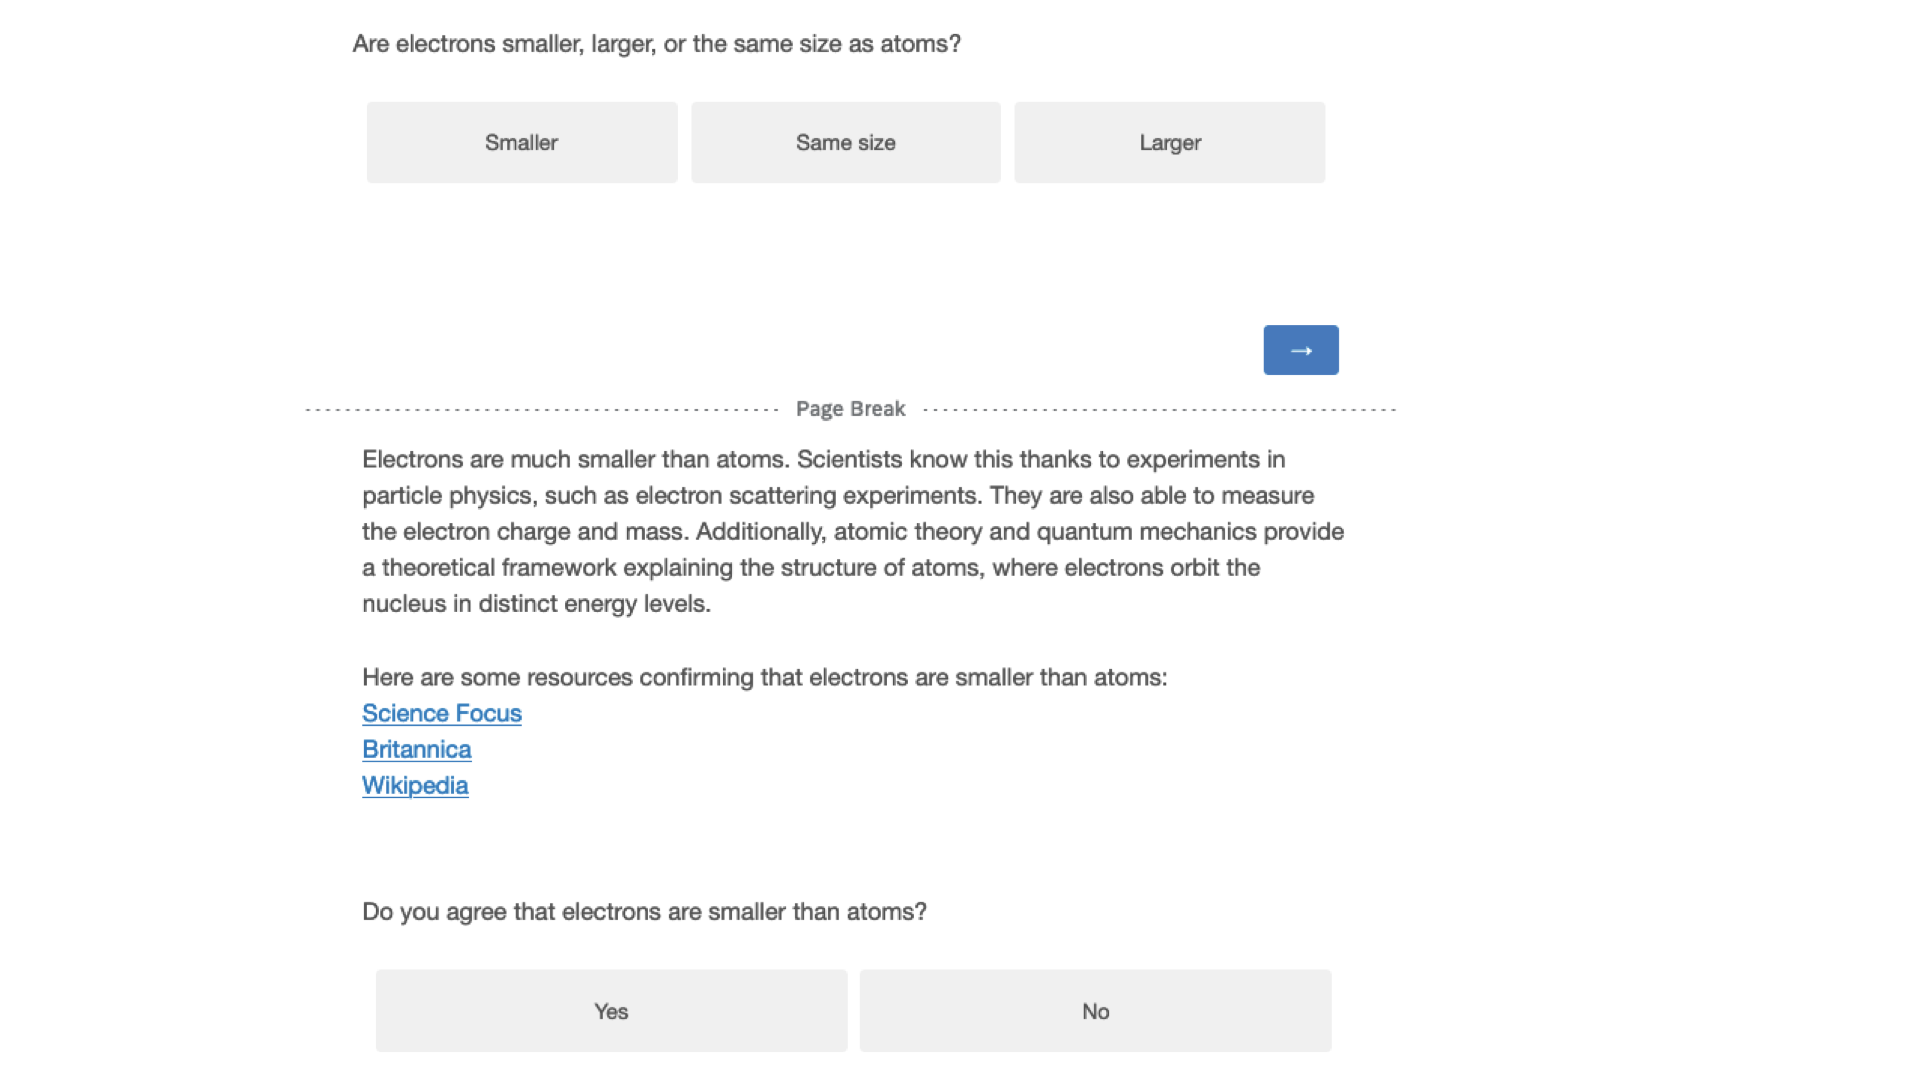
\includegraphics[width=1\linewidth]{./figures/study2_question_example} \hfill{}

\caption{Example of a science question, the scientific consensus and corresponding explanation and sources.}\label{fig:exp2-stimulus-example}
\end{figure}

\subsubsection{Materials}\label{materials-1}

We relied on the same items as in experiment 1. The only difference was that we removed the question on trees.

\subsection{Results}\label{results-1}

As in experiment 1, we find a positive but small correlation between science knowledge and trust in science (H1a: r = 0.28, p \textless{} .001) and a small negative correlation between science knowledge and conspiracy thinking (H2a: r = -0.40, p \textless{} .001). By contrast to experiment 1, we conditioned on initially false answers when looking at the relationship of consensus acceptance with trust in science and conspiracy thinking, respectively. For trust in science, we find no statistically significant correlation (r = 0.16, p = 0.051). For conspiracy thinking we find a small negative one (r = -0.22, p = 0.006).



\begin{figure}
\centering
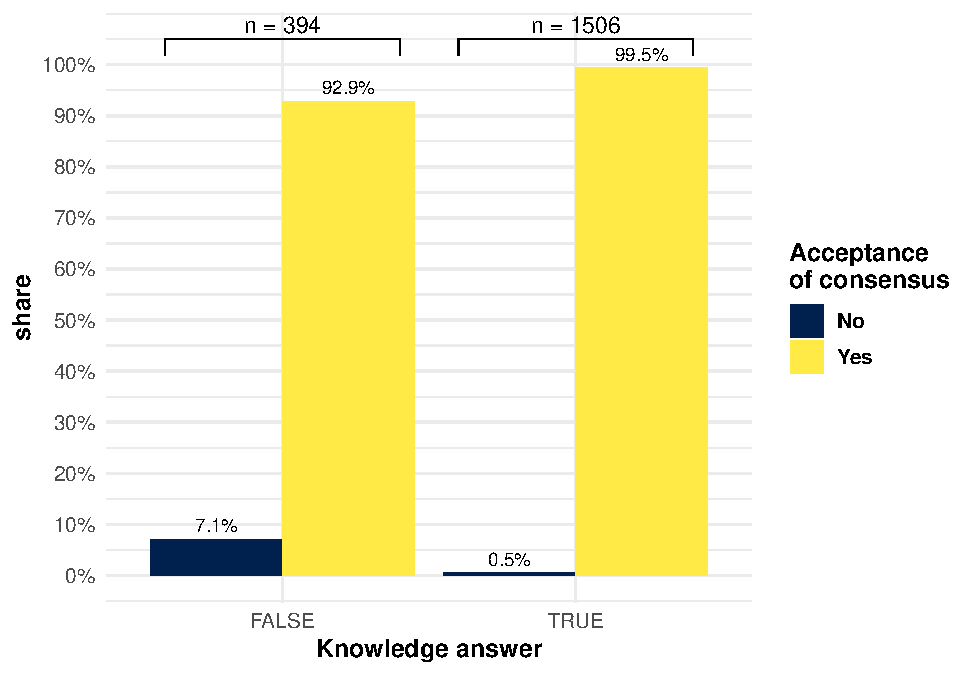
\includegraphics{output/figures/exp2-conditional-acceptance.pdf}
\caption{\label{fig:exp2-conditional-acceptance}Acceptance rates of scientific consensus, based on whether the initial response to the knowledge question was false or true.}
\end{figure}

Confirming results from experiment 1, we find that the more people are knowledgeable about science and the more they tend to accept the scientific consensus even when they are not that knowledgeable in science, the more they tend to trust science. These correlations are relatively weak, which might be partly due to ceiling effects: As illustrated in Fig. \ref{fig:exp2-plot}, (i) most people do trust science, and (ii) that is true even among people with low knowledge or acceptance rates. In Appendix \ref{exp2} we show that these results hold for our alternative measures of trust and conspiracy thinking. We also include more descriptive statistics, such as knowledge and acceptance by science questions.

Regarding RQ1, participants answered on average 79 \% (sd = 0.19) of the questions correctly, and accepted the scientific consensus on average for 98 \% (sd = 0.05) of the questions. Fig. \ref{fig:exp2-conditional-acceptance} illustrates the relationship between knowledge and acceptance. In response to RQ2, in most cases (92.9 \%), participants readily accepted the scientific consensus after having initially given the wrong answer to a question. In very few cases (0.5 \%), participants who gave the correct response afterwards rejected the scientific consensus, thereby contradicting their own initial response.



\begin{figure}
\centering
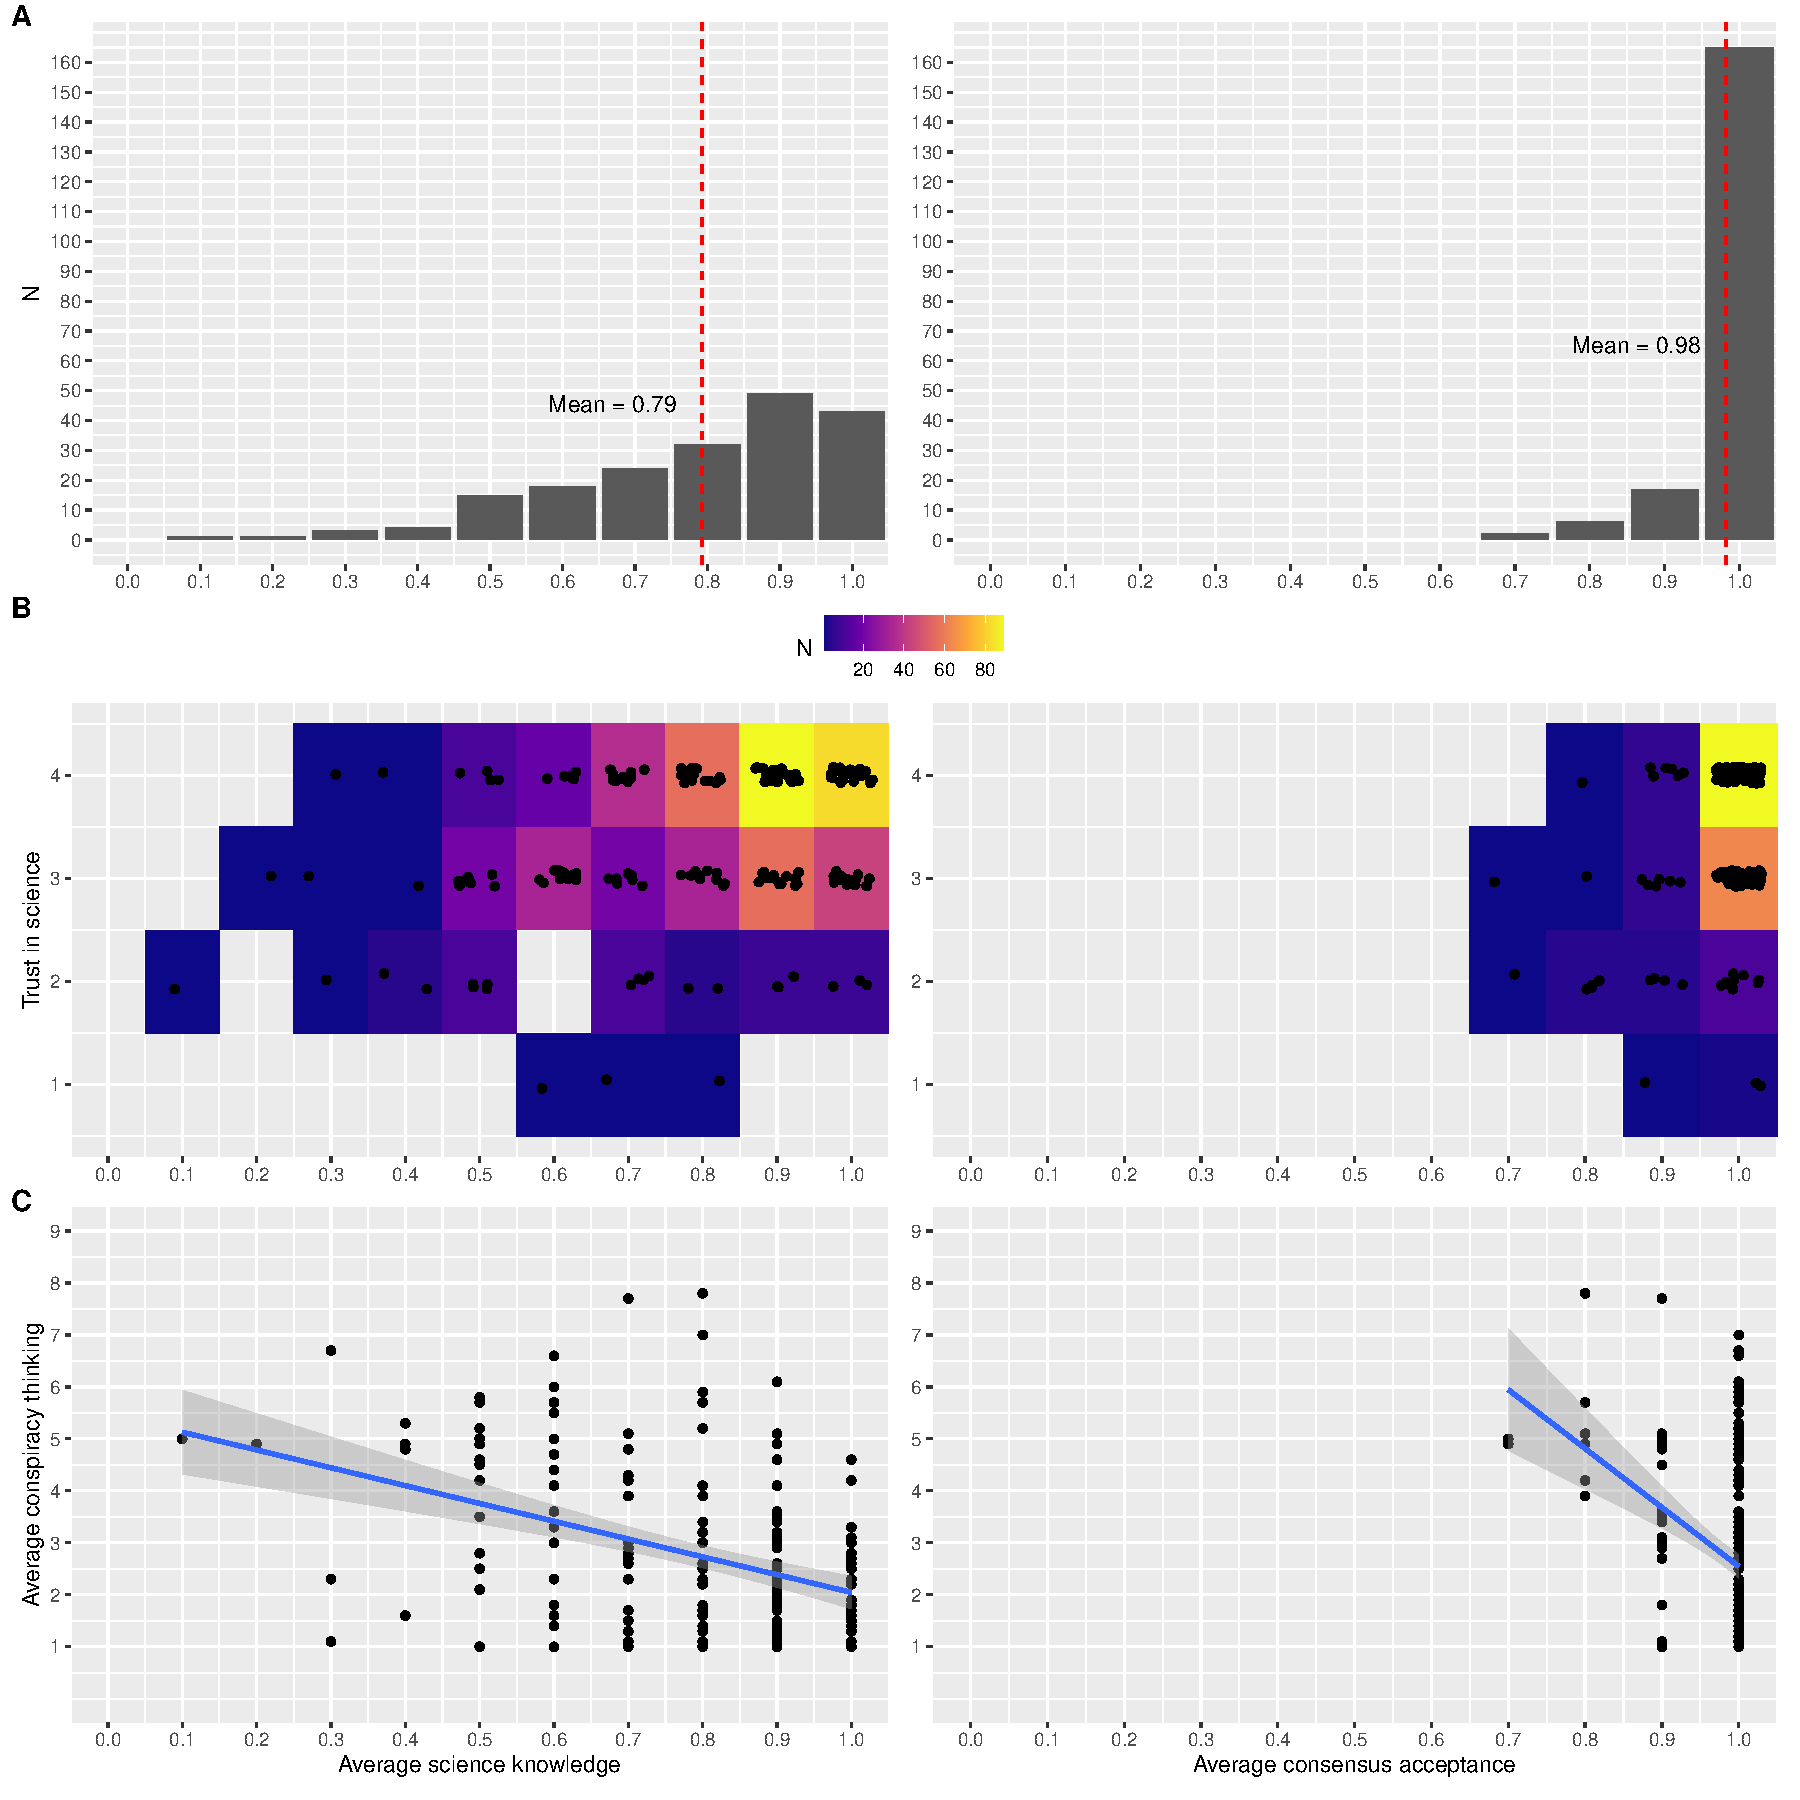
\includegraphics{output/figures/exp2-plot.pdf}
\caption{\label{fig:exp2-plot}\textbf{A} Shows the distribution of science knowledge (left) and acceptance of scientific consensus for participants who gave the wrong answer \textbf{B} Shows the relationship between trust in science and science knowledge/acceptance (if wrong at first, rounded to the first digit) of scientific consensus \textbf{C} Shows the relationship between conspiracy thinking and science knowledge/acceptance (if wrong at first) of scientific consensus}
\end{figure}

For RQ3, we got 35 answers from 25 different participants to the open-ended questions on why they had rejected the scientific consensus on a particular question. Table \ref{tab:exp2-justifications} summarizes these answers by five categories. All answers can be read in Appendix \ref{exp2}.

\begin{table}[tbp]

\begin{center}
\begin{threeparttable}

\caption{\label{tab:exp2-justifications}Justifications by category}

\begin{tabular}{llll}
\toprule
Category & \multicolumn{1}{c}{N (instances)} & \multicolumn{1}{c}{Share (instances)} & \multicolumn{1}{c}{N (unique participants)}\\
\midrule
Personal convictions & 12.00 & 34.3\% & 8.00\\
Mistake & 9.00 & 25.7\% & 8.00\\
No justification & 7.00 & 20\% & 5.00\\
Not convinced & 5.00 & 14.3\% & 5.00\\
Religious Beliefs & 2.00 & 5.7\% & 2.00\\
\bottomrule
\end{tabular}

\end{threeparttable}
\end{center}

\end{table}

\subsection{Discussion}\label{discussion-1}

Similar to experiment 1, most people (i) do know and agree with the scientific consensus, and (ii) tend to accept the scientific consent even if they were not previously aware of it (i.e.~answered the knowledge question wrongly). The share of these latter is considerably larger in experiment 2 (92.9 \%) than in experiment 1 (76.3 \%). While this could be just sampling variation, it might be that adding explanations and sources convinced people more than merely stating the consensus. We also show, again, that people with lower trust in science and who believe more in conspiracy theories tend to both know less about science and accept the scientific consensus less.

\section{Experiment 3}\label{experiment-3}

Study 3 is essentially a replication-\/--with some minor modifications-\/--of study 2, but on a different type of sample. Both study 1 and 2 were run on convenience samples. For study 3, we recruited a sample of people holding anti-vaccination beliefs (see below). By contrast to study 2, after asking participants an open question about why they did not accept the consensus (in cases where they didn't), we provide them with an explicit opportunity to change their answer (Fig. \ref{fig:exp3-explanation-example}). Based on the answers to the open-ended questions, we also pre-registered a categorization scheme of reasons why people rejected the consensus. Finally, we also ask participants about why they agree with the scientific consensus on certain questions, in case they do. We want to know if participants perceive that this is because of trust, or other factors.

As for study 2 (but without conditioning on wrong answers, as we did in study 1), we had the following hypotheses:

\textbf{H1a: Higher trust in science is associated with more science knowledge?}

\textbf{H1b: Higher trust in science is associated with more acceptance of the scientific consensus.}

\textbf{H2a: Higher conspiracy thinking is associated with less science knowledge?}

\textbf{H2b: Higher conspiracy thinking is associated with less acceptance of the scientific consensus.}

We had the following research questions:

\textbf{RQ1: What is the average science knowledge score?}

\textbf{RQ2: What is the average acceptance of the scientific consensus}

\textbf{RQ3: What reasons do participants provide to justify their rejection of the scientific consensus?}

\textbf{RQ4: In case they agree with the scientific consensus, do people feel that this is because of trust?}

\subsection{Methods}\label{methods-2}

\subsubsection{Participants}\label{participants-2}

We recruited 200 participants from the US via prolific, of which none failed our attention check, resulting in a final sample of 200 participants (125 female, 73 male; \(age_\text{mean}\): 42.90, \(age_\text{sd}\): 12.00, \(age_\text{median}\): 41). Since we did not have any prior assumptions on effect sizes and our analyses were descriptive, we did not do a power analysis.

However, due to a randomization mistake for our outcomes, participant answered only two of the three outcome measure blocs (trust in science, conspiracy thinking, and reason for accepting consensus). This leaves us with reduced sample sizes for all analyses concerning these outcomes (N = 140 for trust in science, N = 138 for conspiracy measures, N = 122 for reason for accepting consensus).

\subsubsection{Procedure}\label{procedure-2}

The procedure was mostly the same as in experiment 2. In addition, after each open-ended question on cases where participants rejected the scientific consensus, participants were also asked if they want to change their answer and accept the scientific consensus. Finally, at the end of the survey, we asked participants: ``For the questions in which you agreed with the scientific consensus, would you say that\ldots?'' The answer options were: (i) ``You mostly agree with the consensus because, on that question, you trust scientists'', (ii) ``You mostly agree with the consensus because you have been able to independently verify it'', and (iii) ``Other'', with a text box for participants to explain. Participants who selected ``You mostly agree with the consensus because you have been able to independently verify it'', were asked the open-ended follow-up question: ``Could you please tell us how you independently verified the information?''.



\begin{figure}

{\centering 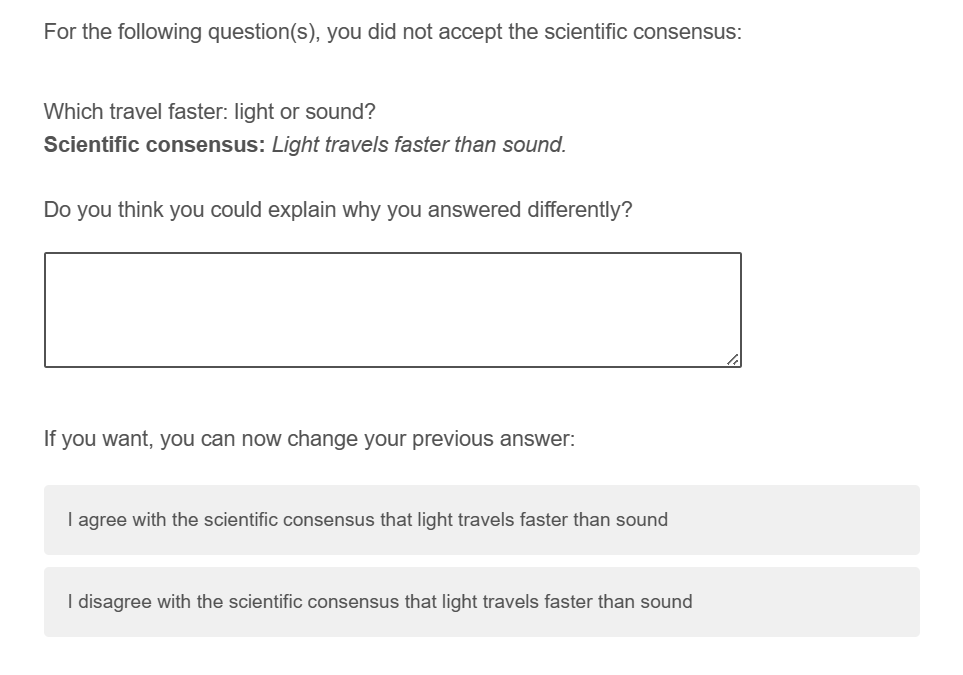
\includegraphics[width=0.5\linewidth]{figures/study3_example_explanation} 

}

\caption{Example of an explanation question and the opportunity to change the previous answer.}\label{fig:exp3-explanation-example}
\end{figure}

\subsubsection{Materials}\label{materials-2}

We relied on the same items as in experiment 2. We used a pre-registered categorization scheme for the open ended answers for why people reject the consensus. The categories were XX and XX. {[}Describe coding process, with independent reviewer etc.{]}

\subsection{Results}\label{results-2}

As in study 1 and 2, we find that participants answered on average 75 \% (sd = 0.18) of the questions correctly, and initially accepted the scientific consensus on average for 96 \% (sd = 0.08) of the questions (RQ2). The acceptance rate is even higher when accounting for opinion revisions towards acceptance of the consensus, after initial rejection (98 \%, sd = 0.06).

Fig. \ref{fig:exp3-conditional-acceptance} illustrates the relationship between knowledge and acceptance. In most cases (87 \%), participants readily accepted the scientific consensus right after having given the wrong answer to a question. After providing the chance to revise the initial consensus rejection, this share is even larger (95.5 \%). In very few cases (0.9 \%), participants who initially gave the correct response afterwards rejected the scientific consensus right after, thereby contradicting their own initial response. This share drops slightly after providing the chance to revise the initial consensus rejection (0.7 \%).

In the appendix XX we provide an analysis that this drop is statistically significant {[}TO DO{]}.

For all correlations, we include opinion revisions for measuring consensus acceptance. We find no statistically significant correlation between science knowledge and trust in science (r = 0.14, p = 0.100), but a samll positive correlation between acceptance of scientific consensus and trust in science (r = 0.20, p = 0.019). Again, these findings might be partly due to ceiling effects: As illustrated in Fig. \ref{fig:exp3-plot}, (i) most people do trust science, and (ii) that is true even among people with low knowledge or acceptance rates. We find no statistically significant correlation between conspiracy thinking and science knowledge (r = -0.16, p = 0.055), and between conspiracy thinking and acceptance of scientific consensus (r = c(cor = -0.023), c(t = -0.27), = 0.788, c(df = 136), -0.189, 0.145, Pearson's product-moment correlation, two.sided, {[}-0.189, 0.145{]}, p = 0.788).

In Appendix \ref{exp3}, we show that these associations are statistically significant (except the last one?). We show that they are robust when using alternative measures of trust and conspiracy thinking. Appendix \ref{exp3} also includes more descriptive statistics, such as knowledge and acceptance by science questions.



\begin{figure}
\centering
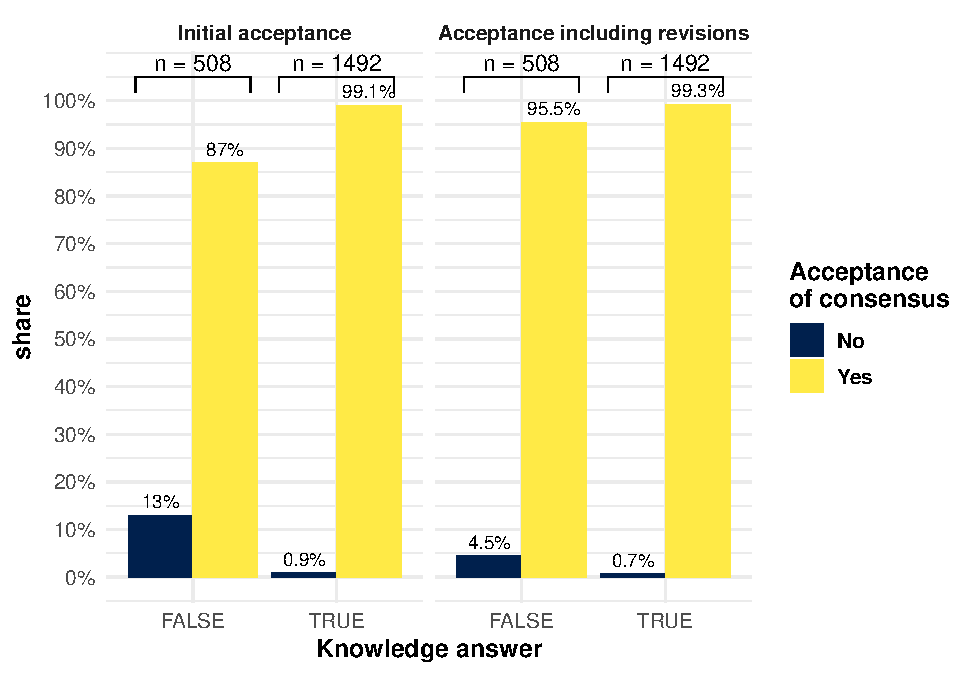
\includegraphics{output/figures/exp3-conditional-acceptance.pdf}
\caption{\label{fig:exp3-conditional-acceptance}Acceptance rates of scientific consensus, based on whether the initial response to the knowledge question was false or true.}
\end{figure}

Regarding RQ1, participants answered on average 75 \% (sd = 0.18) of the questions correctly. For RQ3, we got 74 answers from 47 different participants to the open-ended questions on why they had rejected the scientific consensus on a particular question. Table \ref{tab:exp3-justifications} summarizes these answers by five categories.

All answers can be read in the appendix.

\begin{table}[tbp]

\begin{center}
\begin{threeparttable}

\caption{\label{tab:exp3-justifications}Justifications by category}

\begin{tabular}{llll}
\toprule
Category & \multicolumn{1}{c}{N (instances)} & \multicolumn{1}{c}{Share (instances)} & \multicolumn{1}{c}{N (unique participants)}\\
\midrule
Personal convictions & 25.00 & 33.8\% & 19.00\\
Mistake & 21.00 & 28.4\% & 18.00\\
No justification & 18.00 & 24.3\% & 13.00\\
Not convinced & 7.00 & 9.5\% & 3.00\\
Religious Beliefs & 3.00 & 4.1\% & 3.00\\
\bottomrule
\end{tabular}

\end{threeparttable}
\end{center}

\end{table}

For RQ4, we had 122 participants answering the question. Of these 41.8\% said they accepted the scientific consensus because they trust scientists on this question, while 47.5\% said they independently verified the fact. 10.7\% answered with other ``other'' and gave an open-ended explanation (see Appendix).

We also asked all 58 participants who answered that they had independently verified the answer to explain how they did so. The open-ended answers are listed in Appendix XX.



\begin{figure}
\centering
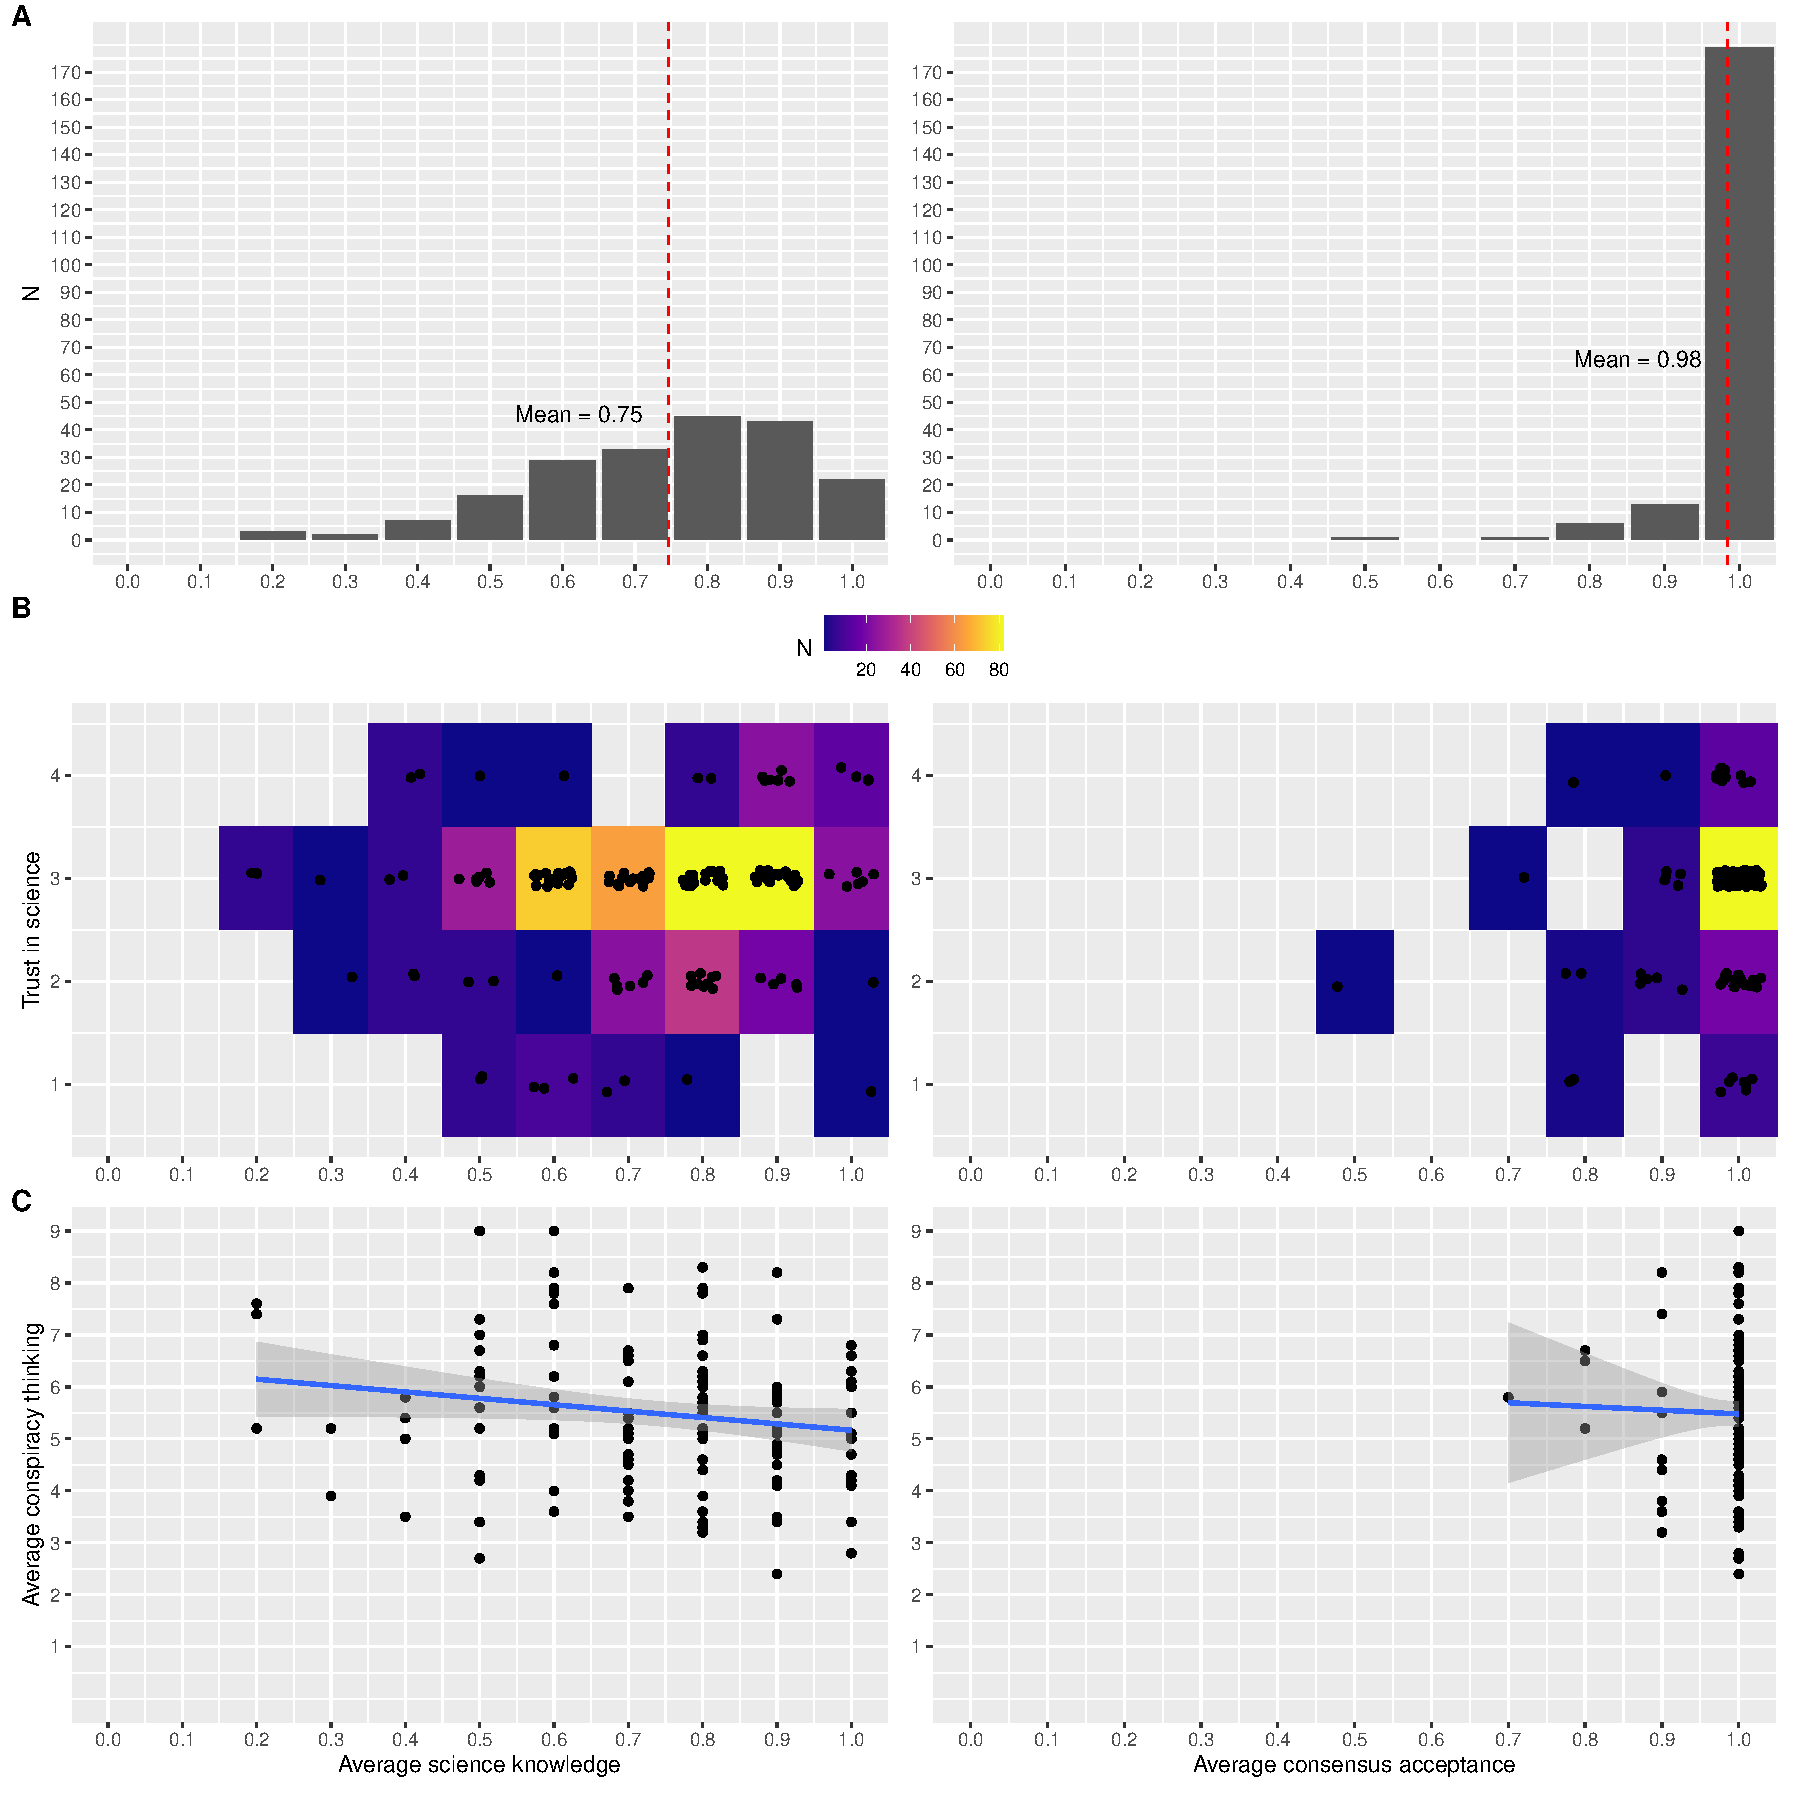
\includegraphics{output/figures/exp3-plot.pdf}
\caption{\label{fig:exp3-plot}\textbf{A} Shows the distribution of science knowledge (left) and acceptance of scientific consensus for participants who gave the wrong answer \textbf{B} Shows the relationship between trust in science and science knowledge/acceptance (if wrong at first, rounded to the first digit) of scientific consensus \textbf{C} Shows the relationship between conspiracy thinking and science knowledge/acceptance (if wrong at first) of scientific consensus}
\end{figure}

\FloatBarrier

\section{References}\label{references}

\phantomsection\label{refs}
\begin{CSLReferences}{1}{0}
\bibitem[\citeproctext]{ref-bruderMeasuringIndividualDifferences2013}
Bruder, M., Haffke, P., Neave, N., Nouripanah, N., \& Imhoff, R. (2013). Measuring individual differences in generic beliefs in conspiracy theories across cultures: Conspiracy mentality questionnaire. \emph{Frontiers in Psychology}, \emph{4}. Retrieved from \url{https://www.frontiersin.org/articles/10.3389/fpsyg.2013.00225}

\bibitem[\citeproctext]{ref-colognaTrustScientistsTheir2024}
Cologna, V., Mede, N. G., Berger, S., Besley, J., Brick, C., Joubert, M., \ldots{} Linden, D. S. van der. (2024). \emph{Trust in scientists and their role in society across 67 countries}. \url{https://doi.org/10.31219/osf.io/6ay7s}

\bibitem[\citeproctext]{ref-lantianMeasuringBeliefConspiracy2016}
Lantian, A., Muller, D., Nurra, C., \& Douglas, K. M. (2016). Measuring Belief in Conspiracy Theories: Validation of a French and English Single-Item Scale. \emph{International Review of Social Psychology}, \emph{29}(1), 1. \url{https://doi.org/10.5334/irsp.8}

\bibitem[\citeproctext]{ref-pennycookOverconfidentlyConspiratorialConspiracy2022}
Pennycook, G., Binnendyk, J., \& Rand, D. (2022). \emph{Overconfidently conspiratorial: Conspiracy believers are dispositionally overconfident and massively overestimate how much others agree with them}. \url{https://doi.org/10.31234/osf.io/d5fz2}

\end{CSLReferences}

\newpage

\appendix


\section{Experiment 1}\label{exp1}

\subsection{Materials}\label{materials-3}

\FloatBarrier

\subsubsection{Conspiracy scales}\label{conspiracy-scales-1}

Beside Belief in Conspiracy Theory Inventory (BCTI) by Pennycook et al. (2022) which report in the main study, we also assessed two other consipiracy thinking measures:

\begin{enumerate}
\def\labelenumi{\arabic{enumi}.}
\tightlist
\item
  The conspiracy mentality questionnaire (CMQ) by Bruder et al. (2013):
  I think that . . .
\end{enumerate}

\begin{itemize}
\tightlist
\item
  \ldots{} many very important things happen in the world, which the public is never informed about. - politicians usually do not tell us the true motives for their decisions.
\item
  \ldots{} government agencies closely monitor all citizens.
\item
  \ldots{} events which superficially seem to lack a connection are often the result of secret activities.
\item
  \ldots{} there are secret organizations that greatly influence political decisions.
\end{itemize}

{[}0\% - 100\%; 0 = certainly not, 100 = certain{]}

\begin{enumerate}
\def\labelenumi{\arabic{enumi}.}
\setcounter{enumi}{1}
\tightlist
\item
  The Single Item Conspiracy Beliefs Scale (SICBS) by Lantian et al. (2016) :
\end{enumerate}

\begin{itemize}
\tightlist
\item
  I think that the official version of the events given by the authorities very often hides the truth. {[}1-9; 1 = Completely false, 5 = Unsure, 9 = Completely true{]}
\end{itemize}

\subsubsection{Trust in science}\label{trust-in-science-1}

We rely on three items

\begin{enumerate}
\def\labelenumi{\arabic{enumi}.}
\item
  How much do you trust scientists in this country? Do you trust them a lot, some, not much, or not at all? {[}1 = Not at all, 2 = Not much, 3 = Some, 4 = A lot{]}
\item
  In general, would you say that you trust science a lot, some, not much, or not at all? {[}1 = Not at all, 2 = Not much, 3 = Some, 4 = A lot{]}
\item
  How much confidence do you have in scientists to act in the best interests of the public? {[}1-5; 1 = No confidence at all, 5 = A great deal of confidence{]}
\end{enumerate}

\subsection{Comparing items}\label{comparing-items}

\subsubsection{Conspiracy theories}\label{conspiracy-theories}

Table \ref{tab:correlation-conspiracy} shows the correlations of the three different scales assessing conspiracy thinking.

\begin{table}[h]

\begin{center}
\begin{threeparttable}

\caption{\label{tab:correlation-conspiracy}Correlations of the three different scales assessing conspiracy thinking}

\begin{tabular}{llll}
\toprule
 & \multicolumn{1}{c}{BCTI} & \multicolumn{1}{c}{CMQ} & \multicolumn{1}{c}{SICBS}\\
\midrule
BCTI & 1.00 & 0.58 & 0.56\\
CMQ & 0.58 & 1.00 & 0.77\\
SICBS & 0.56 & 0.77 & 1.00\\
\bottomrule
\end{tabular}

\end{threeparttable}
\end{center}

\end{table}

\subsubsection{Trust in science}\label{trust-in-science-2}

Table \ref{tab:correlation-trust} shows the correlations of the three different items measuring trust in science.

\begin{table}[h]

\begin{center}
\begin{threeparttable}

\caption{\label{tab:correlation-trust}Correlations of the three different items measuring trust in science}

\begin{tabular}{llll}
\toprule
 & \multicolumn{1}{c}{wgm\_sciencegeneral} & \multicolumn{1}{c}{wgm\_scientists} & \multicolumn{1}{c}{pew}\\
\midrule
wgm\_sciencegeneral & 1.00 & 0.85 & 0.75\\
wgm\_scientists & 0.85 & 1.00 & 0.82\\
pew & 0.75 & 0.82 & 1.00\\
\bottomrule
\end{tabular}

\end{threeparttable}
\end{center}

\end{table}

\subsection{Correlations with alternative measures}\label{correlations-with-alternative-measures}

Table \ref{tab:correlations-outcomes} shows the correlations between knowledge and acceptance, respectively, and outcome variables.

\begin{table}[tbp]

\begin{center}
\begin{threeparttable}

\caption{\label{tab:correlations-outcomes}Correlations between knowledge and acceptance, respectively, and outcome variables}

\begin{tabular}{lll}
\toprule
outcome & \multicolumn{1}{c}{Correlation with knowledge} & \multicolumn{1}{c}{Correlation with acceptance}\\
\midrule
BCTI 
(main conspiracy measure) & -0.38 (p< .001) & -0.33 (p< .001)\\
CMQ & -0.11 (p= 0.121) & -0.07 (p= 0.317)\\
SICBS & -0.1 (p= 0.158) & -0.09 (p= 0.213)\\
WGM trust scientists & 0.23 (p= 0.001) & 0.26 (p< .001)\\
WGM trust general 
(main trust measure) & 0.29 (p< .001) & 0.27 (p< .001)\\
PEW trust scientists & 0.16 (p= 0.027) & 0.21 (p= 0.003)\\
\bottomrule
\end{tabular}

\end{threeparttable}
\end{center}

\end{table}

\subsection{Results conditional on false responses}\label{results-conditional-on-false-responses}

Table \ref{tab:false-response-regression} shows the correlations between acceptance and outcome variables based on linear regression models on standardized values.

\begin{table}

\caption{\label{tab:false-response-regression}Based on false response data only, correlations between acceptance and outcome variables based on linear regression models on standardized values}
\centering
\begin{tabular}[t]{lcccccc}
\toprule
  & BCTI\_avg & CMQ\_avg & SICBS & wgm\_scientists & wgm\_sciencegeneral & pew\\
\midrule
(Intercept) & 0.000 & 0.000 & 0.000 & 0.000 & 0.000 & 0.000\\
 & (0.073) & (0.074) & (0.074) & (0.073) & (0.074) & (0.074)\\
avg\_acceptance & -0.139+ & 0.008 & -0.028 & 0.108 & 0.064 & 0.056\\
 & (0.073) & (0.074) & (0.074) & (0.074) & (0.074) & (0.074)\\
\midrule
Num.Obs. & 184 & 184 & 184 & 184 & 184 & 184\\
R2 & 0.019 & 0.000 & 0.001 & 0.012 & 0.004 & 0.003\\
R2 Adj. & 0.014 & -0.005 & -0.005 & 0.006 & -0.001 & -0.002\\
AIC & 523.6 & 527.2 & 527.0 & 525.0 & 526.4 & 526.6\\
BIC & 533.2 & 536.8 & 536.7 & 534.7 & 536.1 & 536.2\\
Log.Lik. & -258.801 & -260.578 & -260.512 & -259.506 & -260.204 & -260.295\\
RMSE & 0.99 & 1.00 & 1.00 & 0.99 & 1.00 & 1.00\\
\bottomrule
\multicolumn{7}{l}{\rule{0pt}{1em}+ p $<$ 0.1, * p $<$ 0.05, ** p $<$ 0.01, *** p $<$ 0.001}\\
\end{tabular}
\end{table}

\subsection{By-question variation}\label{by-question-variation}

\subsubsection{Knowledge}\label{knowledge}



\begin{figure}
\centering
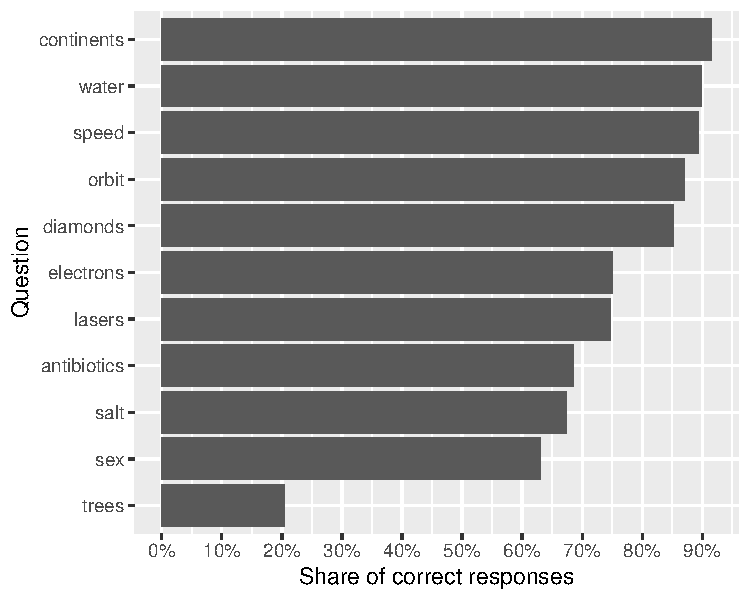
\includegraphics{output/figures/exp1-questions-knowledge.pdf}
\caption{\label{fig:exp1-questions-knowledge}Distribution of correct answers by question.}
\end{figure}

\subsubsection{Acceptance}\label{acceptance}



\begin{figure}
\centering
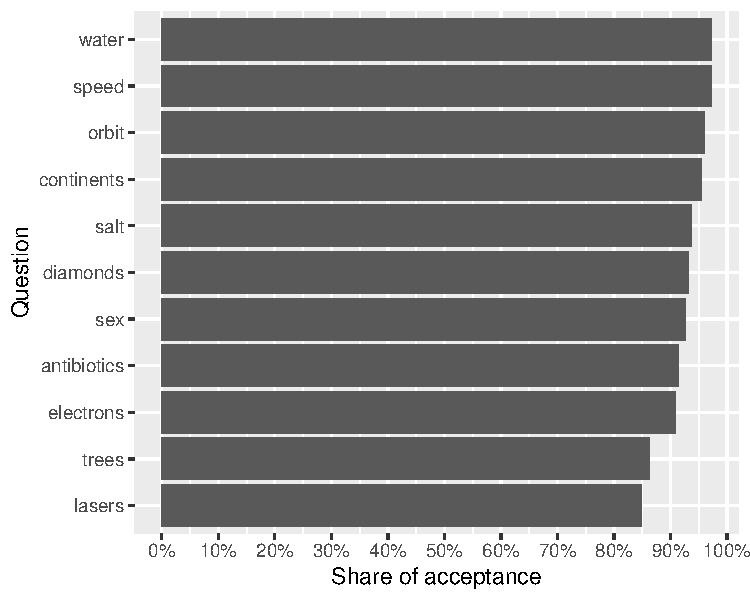
\includegraphics{output/figures/exp1-questions-acceptance.pdf}
\caption{\label{fig:exp1-questions-acceptance}Distribution of consensus acceptance by question.}
\end{figure}

\subsection{Trust in science}\label{trust-in-science-3}



\begin{figure}
\centering
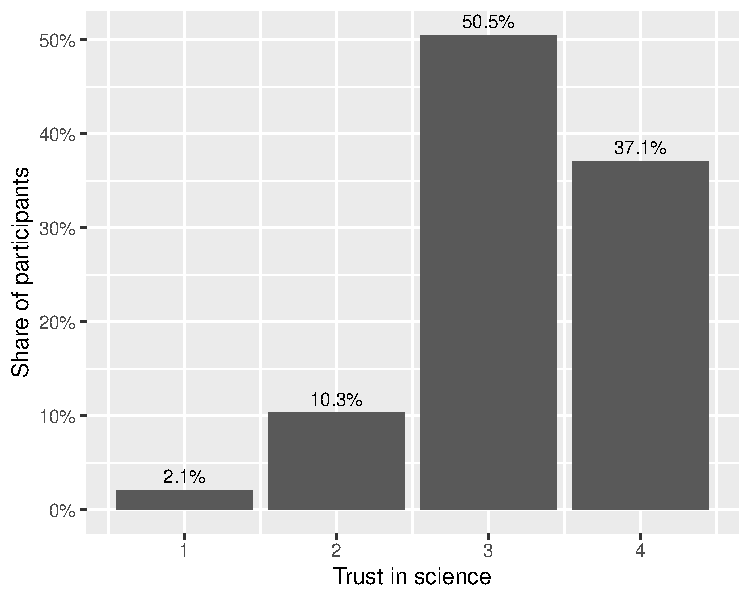
\includegraphics{output/figures/exp1-trust-scientists.pdf}
\caption{\label{fig:exp1-trust-scientists}Distribution of trust in scientists.}
\end{figure}

\subsection{Conspiracy thinking}\label{conspiracy-thinking}

\subsubsection{Distribution}\label{distribution}



\begin{figure}
\centering
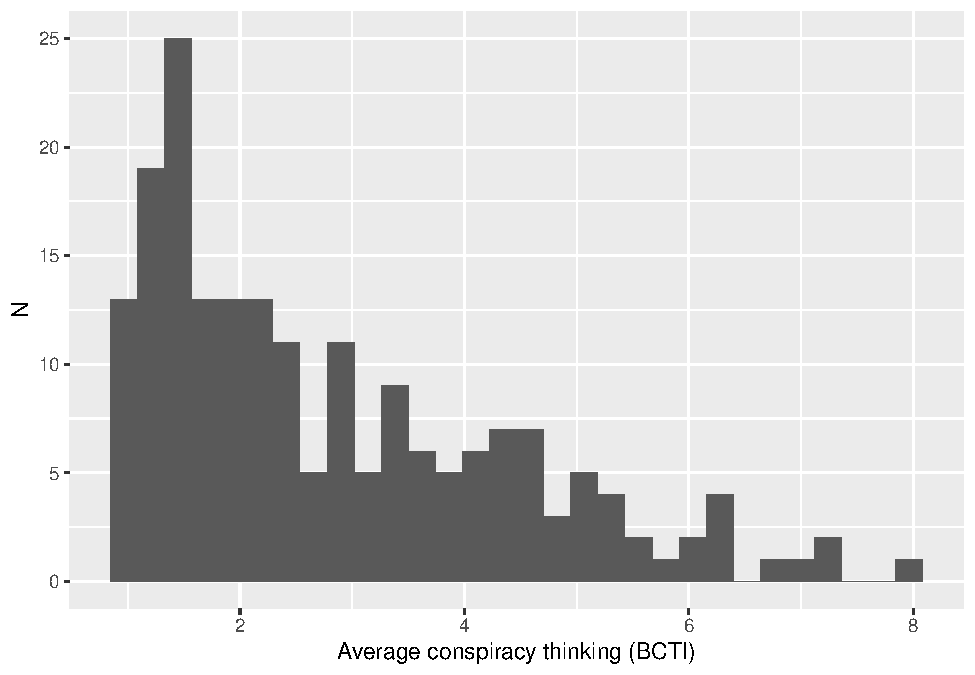
\includegraphics{output/figures/exp1-conspiracy-distribution.pdf}
\caption{\label{fig:exp1-conspiracy-distribution}Distribution of conspiracy thinking.}
\end{figure}

\subsubsection{By-item variation}\label{by-item-variation}



\begin{figure}
\centering
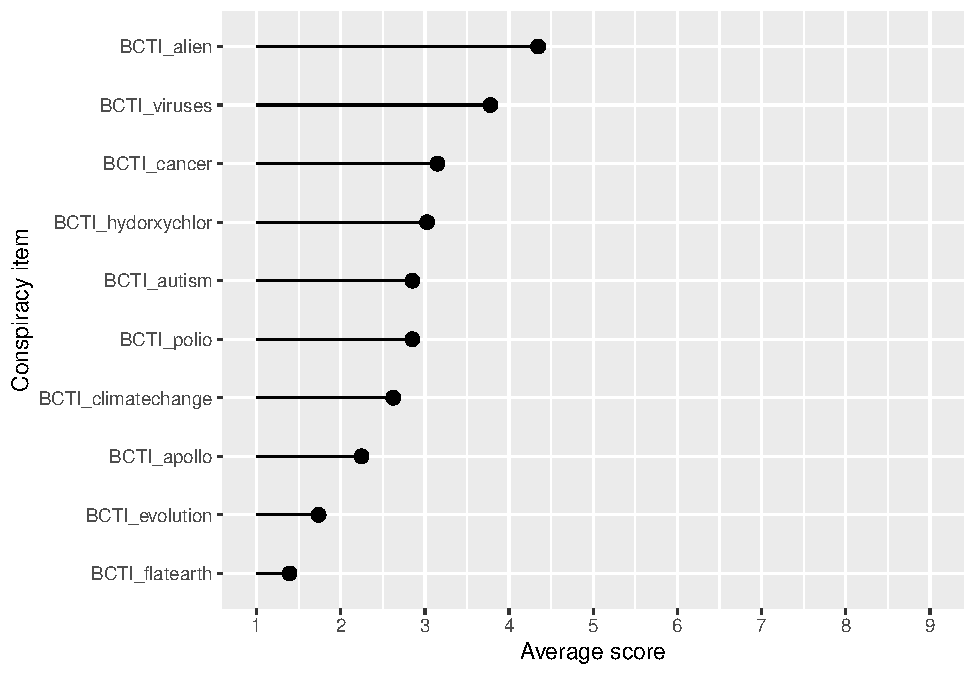
\includegraphics{output/figures/exp1-conspiracy-items.pdf}
\caption{\label{fig:exp1-conspiracy-items}Distribution of conspiracy thinking by item.}
\end{figure}

\subsection{Open ended comments}\label{open-ended-comments}

\begin{longtable}[t]{>{}r>{\raggedright\arraybackslash}p{40em}}
\caption{\label{tab:unnamed-chunk-29}Reasons for consensus rejection}\\
\toprule
id & comments\\
\midrule
1 & no\\
20 & None\\
22 & I answered thoughtfully, good luck!\\
27 & interesting, thank you.\\
30 & n/a\\
\addlinespace
32 & None\\
39 & no\\
41 & none\\
42 & n/a\\
67 & thanks\\
\addlinespace
69 & No comments\\
74 & no\\
76 & none\\
78 & None - thank you!\\
79 & Should've clicked agree about plants getting carbon from the air, but I wanted to look it up first. Whenever I encounter something I didn't know online, I like to cross-reference. In retrospect though, everything else you asked about was simple and on the level, and I'm sure you are correct.

Thanks for your hard work.\\
\addlinespace
84 & No, thank you.\\
86 & n/a\\
89 & N/A\\
95 & no\\
98 & Great topics! Thank you for this study.\\
\addlinespace
109 & To provide context for my responses, I currently study physiology (STEM) and perform academic research as an undergrad at my university.\\
110 & n/a\\
114 & Everything in the survey went fine with no issues. We seem to have a lot of conspiracy theory nuts in the world today and I think it's a sign of the larger mental health crisis that's currently going on.\\
115 & I like the subject content of the survey\\
116 & No\\
\addlinespace
132 & None.\\
133 & very interesting\\
135 & Nope\\
139 & none\\
140 & Air AND water make up the bulk of trees mass and the water is drawn from the earth. Water has much more mass than air and I stand by my answer of Earth being that is where the water is drawn from. The question was very vague and as you see... open to interpretation\\
\addlinespace
141 & n/a\\
148 & no\\
150 & no\\
152 & None.\\
154 & none, tysm!\\
\addlinespace
155 & Not virus, just metals/DDT. And I think it would be impossible for dinosaurs to have sex with the way they are shaped.\\
157 & none\\
159 & I think scientists are acting in the best interests of science rather than the community directly. An unethical scientist could advance scientific knowledge while hurting humanity.\\
161 & Mo Thanks\\
164 & I appreciate science but understand that if scientists don't go along with what investors/govt want they won't receive grants for funding. I also very recently lived through several years of gaslighting about covid. While I realize I'm not the sharpest tool in the shed, I'm not a total idiot. Things that were censored at the beginning of the pandemic are now allowed to be discussed freely. Science should be publicly debated otherwise it isn't science.\\
\addlinespace
165 & it was interesting\\
166 & Everything in the study was good I enjoyed taking it\\
167 & none\\
169 & good study\\
170 & Thanks for the opportunity!\\
\addlinespace
173 & No\\
180 & The study was great.\\
183 & Very interesting study.\\
185 & None\\
186 & Thanks, have  good day\\
\addlinespace
189 & no\\
\bottomrule
\end{longtable}

\clearpage

\section{Experiment 2}\label{exp2}

\subsection{Materials}\label{materials-4}

\FloatBarrier

See Appendix \ref{exp1}.

\subsection{Comparing items}\label{comparing-items-1}

\subsubsection{Conspiracy theories}\label{conspiracy-theories-1}

Table \ref{tab:exp2-correlation-conspiracy} shows the correlations of the three different scales assessing conspiracy thinking.

\begin{table}[h]

\begin{center}
\begin{threeparttable}

\caption{\label{tab:exp2-correlation-conspiracy}Correlations of the three different scales assessing conspiracy thinking}

\begin{tabular}{llll}
\toprule
 & \multicolumn{1}{c}{BCTI} & \multicolumn{1}{c}{CMQ} & \multicolumn{1}{c}{SICBS}\\
\midrule
BCTI & 1.00 & 0.66 & 0.63\\
CMQ & 0.66 & 1.00 & 0.86\\
SICBS & 0.63 & 0.86 & 1.00\\
\bottomrule
\end{tabular}

\end{threeparttable}
\end{center}

\end{table}

\subsubsection{Trust in science}\label{trust-in-science-4}

Table \ref{tab:exp2-correlation-trust} shows the correlations of the three different items measuring trust in science.

\begin{table}[h]

\begin{center}
\begin{threeparttable}

\caption{\label{tab:exp2-correlation-trust}Correlations of the three different items measuring trust in science}

\begin{tabular}{llll}
\toprule
 & \multicolumn{1}{c}{wgm\_sciencegeneral} & \multicolumn{1}{c}{wgm\_scientists} & \multicolumn{1}{c}{pew}\\
\midrule
wgm\_sciencegeneral & 1.00 & 0.89 & 0.79\\
wgm\_scientists & 0.89 & 1.00 & 0.85\\
pew & 0.79 & 0.85 & 1.00\\
\bottomrule
\end{tabular}

\end{threeparttable}
\end{center}

\end{table}

\subsection{Correlations with alternative measures}\label{correlations-with-alternative-measures-1}

Table \ref{tab:exp2-correlations-outcomes} shows the correlations between knowledge and acceptance, respectively, and outcome variables.

\begin{table}[tbp]

\begin{center}
\begin{threeparttable}

\caption{\label{tab:exp2-correlations-outcomes}Correlations between knowledge and acceptance, respectively, and outcome variables}

\begin{tabular}{lllllllll}
\toprule
std.error & \multicolumn{1}{c}{statistic} & \multicolumn{1}{c}{p.value} & \multicolumn{1}{c}{conf.low} & \multicolumn{1}{c}{conf.high} & \multicolumn{1}{c}{outcome} & \multicolumn{1}{c}{ci} & \multicolumn{1}{c}{Correlation with knowledge} & \multicolumn{1}{c}{Correlation with acceptance}\\
\midrule
0.07 & -6.01 & < .001 & -0.53 & -0.27 & BCTI 
(main conspiracy measure) & {}[-0.533, -0.27] & -0.40 & NA\\
0.07 & -2.36 & = 0.019 & -0.31 & -0.03 & CMQ & {}[-0.311, -0.028] & -0.17 & NA\\
0.07 & -1.91 & = 0.058 & -0.28 & 0.00 & SICBS & {}[-0.28, 0.005] & -0.14 & NA\\
0.07 & 3.20 & = 0.002 & 0.09 & 0.37 & WGM trust scientists & {}[0.087, 0.368] & 0.23 & NA\\
0.07 & 3.98 & < .001 & 0.14 & 0.42 & WGM trust general 
(main trust measure) & {}[0.14, 0.417] & 0.28 & NA\\
0.07 & 2.23 & = 0.027 & 0.02 & 0.30 & PEW trust scientists & {}[0.019, 0.303] & 0.16 & NA\\
0.07 & -5.47 & < .001 & -0.50 & -0.24 & BCTI 
(main conspiracy measure) & {}[-0.504, -0.237] & NA & -0.37\\
0.07 & -3.03 & = 0.003 & -0.36 & -0.08 & CMQ & {}[-0.356, -0.076] & NA & -0.22\\
0.07 & -2.76 & = 0.006 & -0.34 & -0.06 & SICBS & {}[-0.338, -0.056] & NA & -0.20\\
0.07 & 3.51 & < .001 & 0.11 & 0.39 & WGM trust scientists & {}[0.108, 0.387] & NA & 0.25\\
0.07 & 4.29 & < .001 & 0.16 & 0.44 & WGM trust general 
(main trust measure) & {}[0.161, 0.436] & NA & 0.30\\
0.07 & 3.04 & = 0.003 & 0.08 & 0.36 & PEW trust scientists & {}[0.076, 0.357] & NA & 0.22\\
\bottomrule
\end{tabular}

\end{threeparttable}
\end{center}

\end{table}

\subsection{Results conditional on false responses}\label{results-conditional-on-false-responses-1}

Table \ref{tab:exp2-false-response-regression} shows the correlations between acceptance and outcome variables based on linear regression models on standardized values.

\begin{table}

\caption{\label{tab:exp2-false-response-regression}Based on false response data only, correlations between acceptance and outcome variables based on linear regression models on standardized values}
\centering
\begin{tabular}[t]{lcccccc}
\toprule
  & BCTI\_avg & CMQ\_avg & SICBS & wgm\_scientists & wgm\_sciencegeneral & pew\\
\midrule
(Intercept) & 0.000 & 0.000 & 0.000 & 0.000 & 0.000 & 0.000\\
 & (0.081) & (0.080) & (0.081) & (0.082) & (0.082) & \vphantom{1} (0.082)\\
avg\_acceptance & -0.225** & -0.247** & -0.201* & 0.131 & 0.161+ & 0.130\\
 & (0.081) & (0.080) & (0.081) & (0.082) & (0.082) & (0.082)\\
\midrule
Num.Obs. & 147 & 147 & 147 & 147 & 147 & 147\\
R2 & 0.051 & 0.061 & 0.041 & 0.017 & 0.026 & 0.017\\
R2 Adj. & 0.044 & 0.054 & 0.034 & 0.010 & 0.019 & 0.010\\
AIC & 414.5 & 412.9 & 416.1 & 419.6 & 418.3 & 419.7\\
BIC & 423.5 & 421.9 & 425.0 & 428.6 & 427.3 & 428.6\\
Log.Lik. & -204.248 & -203.465 & -205.036 & -206.802 & -206.141 & -206.826\\
RMSE & 0.97 & 0.97 & 0.98 & 0.99 & 0.98 & 0.99\\
\bottomrule
\multicolumn{7}{l}{\rule{0pt}{1em}+ p $<$ 0.1, * p $<$ 0.05, ** p $<$ 0.01, *** p $<$ 0.001}\\
\end{tabular}
\end{table}

\subsection{By-question variation}\label{by-question-variation-1}

\subsubsection{Knowledge}\label{knowledge-1}



\begin{figure}
\centering
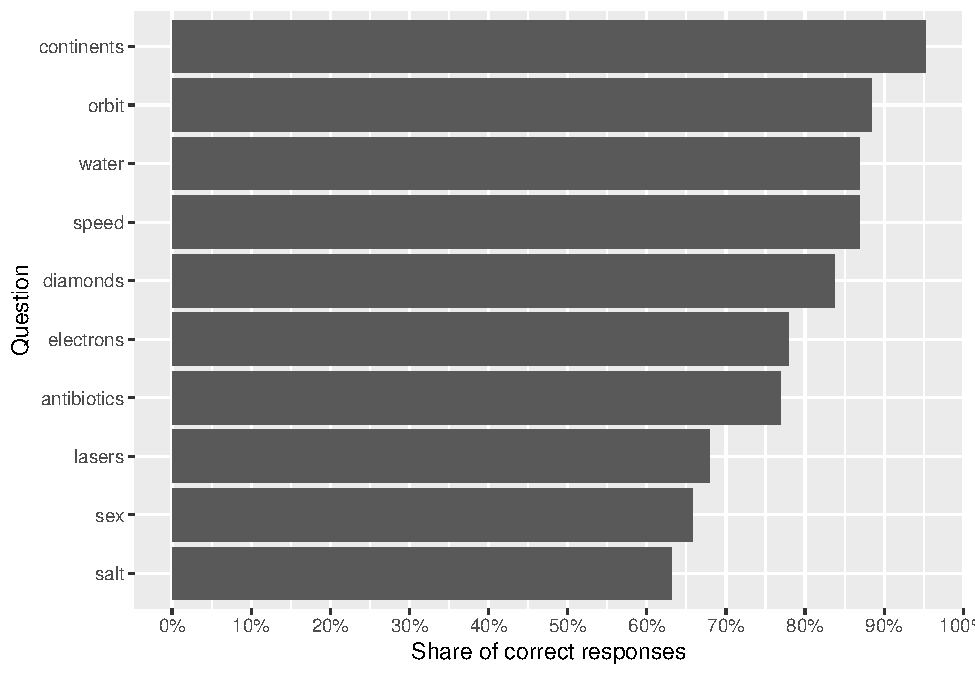
\includegraphics{output/figures/exp2-questions-knowledge.pdf}
\caption{\label{fig:exp2-questions-knowledge}Distribution of correct answers by question.}
\end{figure}

\subsubsection{Acceptance}\label{acceptance-1}



\begin{figure}
\centering
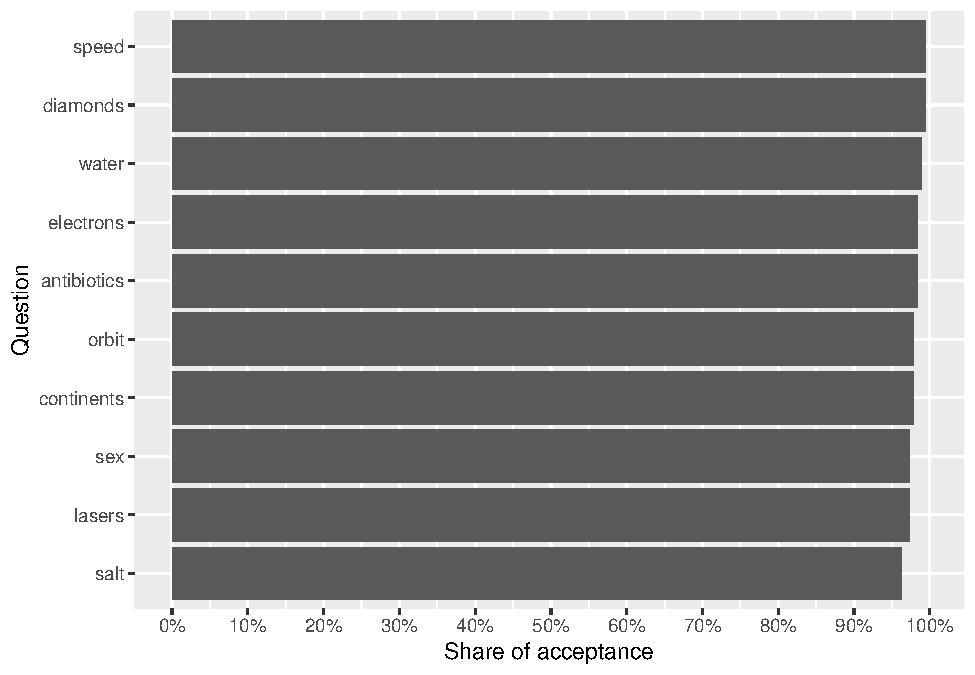
\includegraphics{output/figures/exp2-questions-acceptance.pdf}
\caption{\label{fig:exp2-questions-acceptance}Distribution of consensus acceptance by question.}
\end{figure}

\subsection{Trust in science}\label{trust-in-science-5}



\begin{figure}
\centering
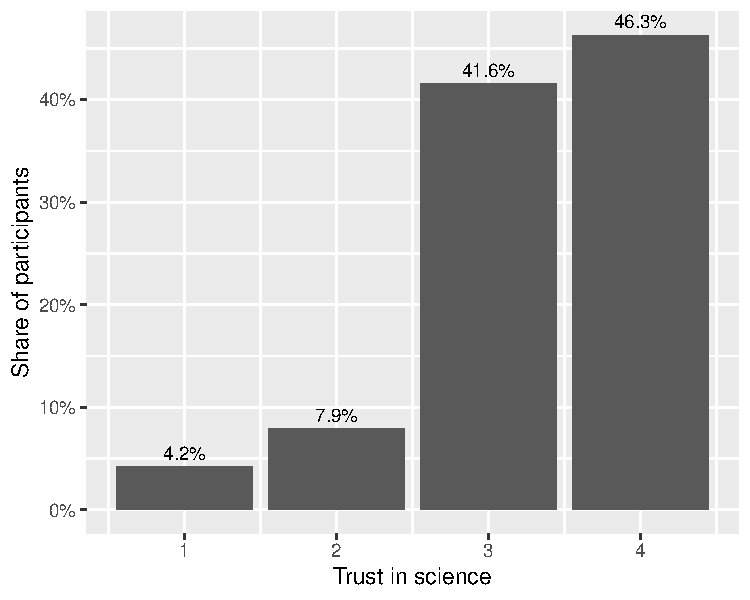
\includegraphics{output/figures/exp2-trust-scientists.pdf}
\caption{\label{fig:exp2-trust-scientists}Distribution of trust in scientists.}
\end{figure}

\subsection{Conspiracy thinking}\label{conspiracy-thinking-1}

\subsubsection{Distribution}\label{distribution-1}



\begin{figure}
\centering
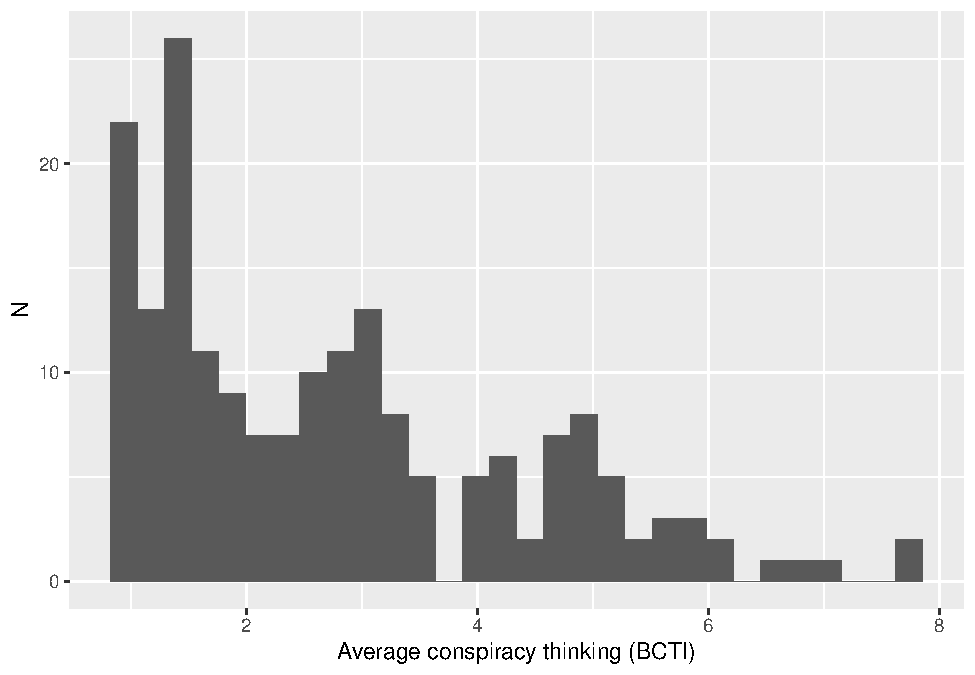
\includegraphics{output/figures/exp2-conspiracy-distribution.pdf}
\caption{\label{fig:exp2-conspiracy-distribution}Distribution of conspiracy thinking.}
\end{figure}

\subsubsection{By-item variation}\label{by-item-variation-1}



\begin{figure}
\centering
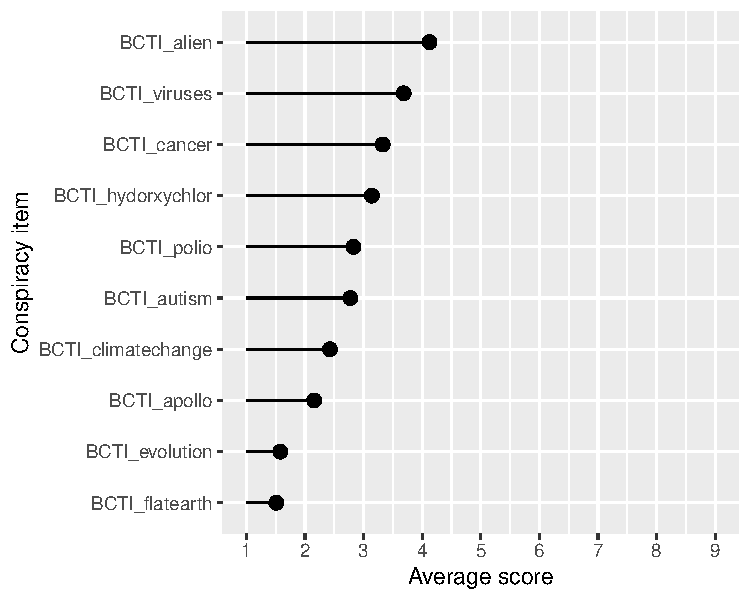
\includegraphics{output/figures/exp2-conspiracy-items.pdf}
\caption{\label{fig:exp2-conspiracy-items}Distribution of conspiracy thinking by item.}
\end{figure}

\subsection{Reasons for consensus rejection}\label{reasons-for-consensus-rejection}

\subsubsection{By category}\label{by-category}

{[}To do{]}

\subsubsection{All raw answers}\label{all-raw-answers}

\begin{longtable}[t]{>{}r>{}l>{\raggedright\arraybackslash}p{30em}}
\caption{\label{tab:exp2-reasons-rejection}Reasons for consensus rejection}\\
\toprule
id & question & answer\\
\midrule
33 & sex & Because I didn't think the information provided here was accurate, more or less.\\
45 & lasers & I read the article.\\
45 & salt & Read the article provided.\\
47 & lasers & The statement "lasers do not work by focusing sound waves" is correct according to scientific consensus. Lasers operate on the principles of stimulated emission of radiation, wherein photons are emitted in a coherent, focused beam through the process of stimulated emission.\\
47 & diamonds & Are diamonds made of carbon? Scientific consensus: Diamonds are made of carbon.  Do you think you could explain why you answered differently?\\
\addlinespace
47 & water & it likely arose from a mistake or miscommunication.\\
50 & orbit & I honestly couldn't remember.\\
50 & speed & When I looked it up I got two different answers.\\
71 & water & After I put "No", I realized that I was thinking about "H2o" incorrectly. So yes, I actually do agree.\\
73 & electrons & Atoms are known to be the smallest unit of matter.\\
\addlinespace
77 & continents & I believe God make it they way it is and if He wanted it changed, He would have done it\\
78 & sex & no\\
78 & salt & no\\
79 & orbit & It’s early and I’m tired. I misread it.\\
105 & salt & I think I simply misunderstood the paragraph. I'm actually trying to read it thoroughly and answering truthfully, but I have misread it.\\
\addlinespace
109 & electrons & Maybe\\
127 & continents & I'm a young earth Christian. I believe the Christian Bible (and outside sources) offers ample evidence that the earth is thousands of years old, not millions.\\
127 & orbit & I do not believe in the heliocentric model of an earth spinning around a centralized sun.\\
130 & continents & I don't think the continent move rather it is the atmosphere\\
130 & sex & I think that the gene both parent release should determine the sex of the baby\\
\addlinespace
131 & antibiotics & There are some antibiotics that also kill viruses\\
132 & salt & Because it says that table salt is not made of calcium carbonate, so I clicked no.\\
133 & lasers & I feel like the excerpt that was provided did not definitively state the answer.\\
140 & lasers & It was confusing to understand the explanation of why lasers don’t focus on sound\\
152 & continents & I think that they were that way after the ice age.  It split apart the whole surface and then water filled in and they have remained the same for ever.  They are not moving around or have they for millions of years.\\
\addlinespace
152 & orbit & The  Earth circles the sun every day.  The dark side is when the moon comes out.  So everyday, you have daylight and dark (moon).  Dark comes from the dark side of the sun.\\
170 & lasers & I may have misread, but I did not see confirmation of this.\\
172 & salt & no\\
178 & electrons & This answer is different because atoms is everywhere and you can't see it but electrons aren't out that as much at all but you could possibly know it's there\\
178 & antibiotics & Because antibiotics can kill bacteria in which kills the virus as well in the process so you get healed with this product\\
\addlinespace
178 & sex & There is no 100\% evidence that this is the case and I still fully believe that it is from both genes to make this decision.\\
179 & antibiotics & Antibiotics seem that if they are capable of killing tiny things such as bacteria then they are most likely to attach to other things in out bodies and cause it harm although unintentional.\\
183 & salt & I thought the scientific consensus was right\\
186 & sex & The scientific consensus is clear: both parents' genes determine the sex of a baby, specifically the sex chromosomes they contribute.\\
189 & salt & I made an error in my selection.\\
\bottomrule
\end{longtable}

\clearpage

\section{Experiment 3}\label{exp3}

\subsection{Materials}\label{materials-5}

\FloatBarrier

See Appendix \ref{exp1}.

\subsection{Comparing items}\label{comparing-items-2}

\subsubsection{Conspiracy theories}\label{conspiracy-theories-2}

Table \ref{tab:exp3-correlation-conspiracy} shows the correlations of the three different scales assessing conspiracy thinking.

\begin{table}[h]

\begin{center}
\begin{threeparttable}

\caption{\label{tab:exp3-correlation-conspiracy}Correlations of the three different scales assessing conspiracy thinking}

\begin{tabular}{llll}
\toprule
 & \multicolumn{1}{c}{BCTI} & \multicolumn{1}{c}{CMQ} & \multicolumn{1}{c}{SICBS}\\
\midrule
BCTI & 1.00 & NA & NA\\
CMQ & NA & 1.00 & NA\\
SICBS & NA & NA & 1.00\\
\bottomrule
\end{tabular}

\end{threeparttable}
\end{center}

\end{table}

\subsubsection{Trust in science}\label{trust-in-science-6}

Table \ref{tab:exp3-correlation-trust} shows the correlations of the three different items measuring trust in science.

\begin{table}[h]

\begin{center}
\begin{threeparttable}

\caption{\label{tab:exp3-correlation-trust}Correlations of the three different items measuring trust in science}

\begin{tabular}{llll}
\toprule
 & \multicolumn{1}{c}{wgm\_sciencegeneral} & \multicolumn{1}{c}{wgm\_scientists} & \multicolumn{1}{c}{pew}\\
\midrule
wgm\_sciencegeneral & 1.00 & NA & NA\\
wgm\_scientists & NA & 1.00 & NA\\
pew & NA & NA & 1.00\\
\bottomrule
\end{tabular}

\end{threeparttable}
\end{center}

\end{table}

\subsection{Correlations with alternative measures}\label{correlations-with-alternative-measures-2}

Table \ref{tab:exp3-correlations-outcomes} shows the correlations between knowledge and acceptance, respectively, and outcome variables.

\begin{table}[tbp]

\begin{center}
\begin{threeparttable}

\caption{\label{tab:exp3-correlations-outcomes}Correlations between knowledge and acceptance, respectively, and outcome variables}

\begin{tabular}{lllllllll}
\toprule
std.error & \multicolumn{1}{c}{statistic} & \multicolumn{1}{c}{p.value} & \multicolumn{1}{c}{conf.low} & \multicolumn{1}{c}{conf.high} & \multicolumn{1}{c}{outcome} & \multicolumn{1}{c}{ci} & \multicolumn{1}{c}{Correlation with knowledge} & \multicolumn{1}{c}{Correlation with acceptance}\\
\midrule
0.08 & -1.93 & = 0.055 & -0.32 & 0.00 & BCTI 
(main conspiracy measure) & {}[-0.317, 0.004] & -0.16 & NA\\
0.08 & 0.10 & = 0.925 & -0.15 & 0.17 & CMQ & {}[-0.154, 0.17] & 0.01 & NA\\
0.08 & 0.30 & = 0.767 & -0.14 & 0.19 & SICBS & {}[-0.138, 0.186] & 0.02 & NA\\
0.08 & 1.31 & = 0.193 & -0.06 & 0.28 & WGM trust scientists & {}[-0.056, 0.276] & 0.11 & NA\\
0.08 & 1.66 & = 0.100 & -0.03 & 0.30 & WGM trust general 
(main trust measure) & {}[-0.027, 0.304] & 0.14 & NA\\
0.08 & -0.91 & = 0.367 & -0.24 & 0.09 & PEW trust scientists & {}[-0.243, 0.09] & -0.08 & NA\\
0.11 & -0.27 & = 0.788 & -0.25 & 0.19 & BCTI 
(main conspiracy measure) & {}[-0.246, 0.187] & NA & -0.03\\
0.11 & -0.08 & = 0.934 & -0.23 & 0.21 & CMQ & {}[-0.226, 0.208] & NA & -0.01\\
0.11 & 0.02 & = 0.987 & -0.22 & 0.22 & SICBS & {}[-0.215, 0.218] & NA & 0.00\\
0.07 & 2.72 & = 0.007 & 0.05 & 0.34 & WGM trust scientists & {}[0.054, 0.343] & NA & 0.20\\
0.07 & 2.37 & = 0.019 & 0.03 & 0.32 & WGM trust general 
(main trust measure) & {}[0.029, 0.32] & NA & 0.17\\
0.07 & 1.64 & = 0.104 & -0.03 & 0.27 & PEW trust scientists & {}[-0.025, 0.268] & NA & 0.12\\
\bottomrule
\end{tabular}

\end{threeparttable}
\end{center}

\end{table}

\subsection{Results conditional on false responses}\label{results-conditional-on-false-responses-2}

Table \ref{tab:exp3-false-response-regression} shows the correlations between acceptance and outcome variables based on linear regression models on standardized values.

\begin{table}

\caption{\label{tab:exp3-false-response-regression}Based on false response data only, correlations between acceptance and outcome variables based on linear regression models on standardized values}
\centering
\begin{tabular}[t]{lcccccc}
\toprule
  & BCTI\_avg & CMQ\_avg & SICBS & wgm\_scientists & wgm\_sciencegeneral & pew\\
\midrule
(Intercept) & -0.001 & 0.000 & 0.000 & 0.005 & 0.002 & 0.008\\
 & (0.091) & (0.091) & (0.091) & (0.088) & (0.089) & (0.088)\\
avg\_acceptance & -0.043 & -0.025 & -0.009 & 0.083 & 0.039 & 0.125\\
 & (0.090) & (0.090) & (0.090) & (0.079) & (0.079) & (0.078)\\
\midrule
Num.Obs. & 122 & 122 & 122 & 128 & 128 & 128\\
R2 & 0.002 & 0.001 & 0.000 & 0.009 & 0.002 & 0.020\\
R2 Adj. & -0.006 & -0.008 & -0.008 & 0.001 & -0.006 & 0.012\\
AIC & 351.0 & 351.1 & 351.2 & 367.1 & 368.0 & 365.7\\
BIC & 359.4 & 359.6 & 359.6 & 375.7 & 376.5 & 374.2\\
Log.Lik. & -172.491 & -172.571 & -172.604 & -180.560 & -180.996 & -179.843\\
RMSE & 0.99 & 1.00 & 1.00 & 0.99 & 1.00 & 0.99\\
\bottomrule
\multicolumn{7}{l}{\rule{0pt}{1em}+ p $<$ 0.1, * p $<$ 0.05, ** p $<$ 0.01, *** p $<$ 0.001}\\
\end{tabular}
\end{table}

\subsection{By-question variation}\label{by-question-variation-2}

\subsubsection{Knowledge}\label{knowledge-2}



\begin{figure}
\centering
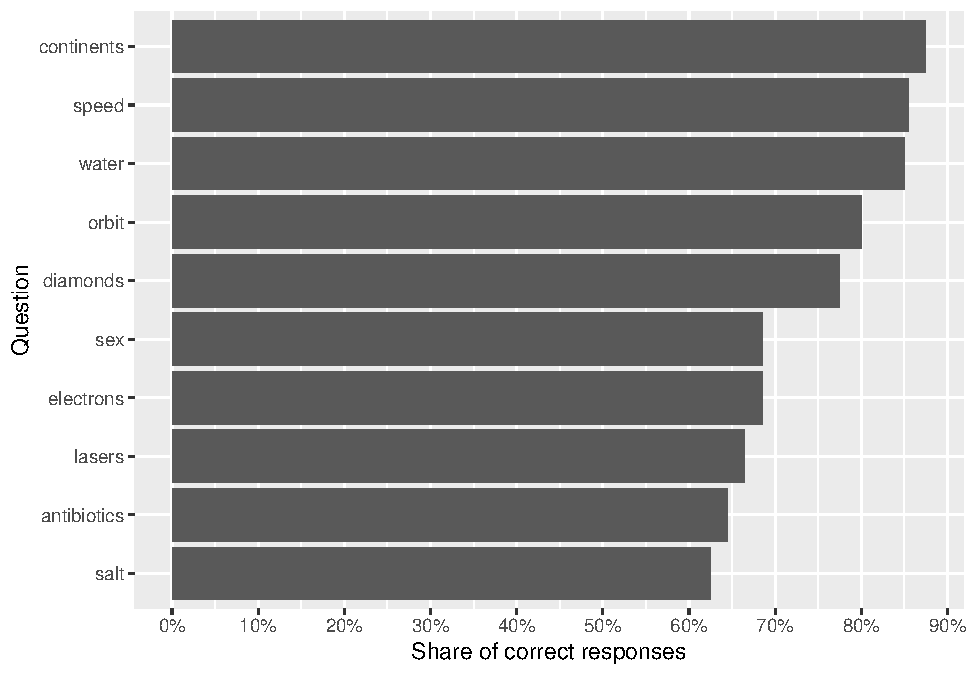
\includegraphics{output/figures/exp3-questions-knowledge.pdf}
\caption{\label{fig:exp3-questions-knowledge}Distribution of correct answers by question.}
\end{figure}



\begin{figure}
\centering
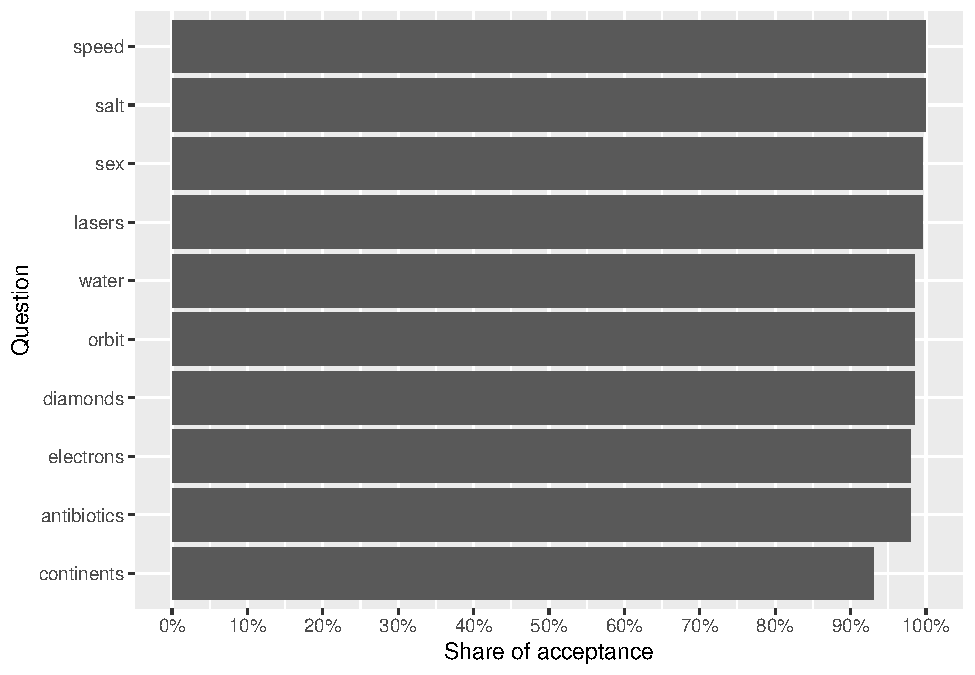
\includegraphics{output/figures/exp3-questions-acceptance.pdf}
\caption{\label{fig:exp3-questions-acceptance}Distribution of consensus acceptance by question.}
\end{figure}

\subsection{Trust in science}\label{trust-in-science-7}



\begin{figure}
\centering
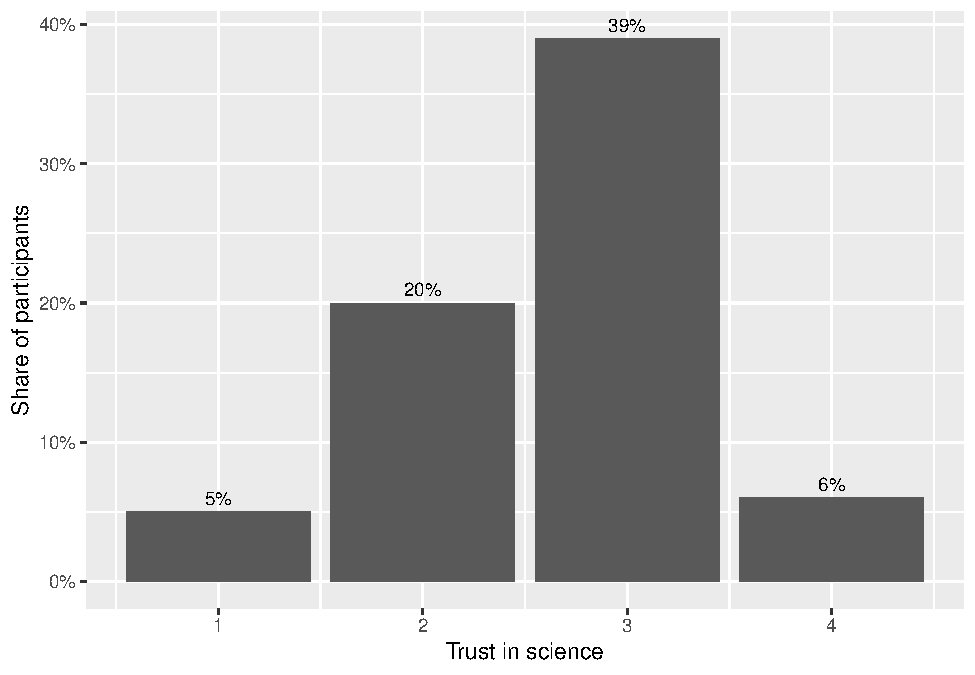
\includegraphics{output/figures/exp3-trust-scientists.pdf}
\caption{\label{fig:exp3-trust-scientists}Distribution of trust in scientists.}
\end{figure}

\subsection{Conspiracy thinking}\label{conspiracy-thinking-2}



\begin{figure}
\centering
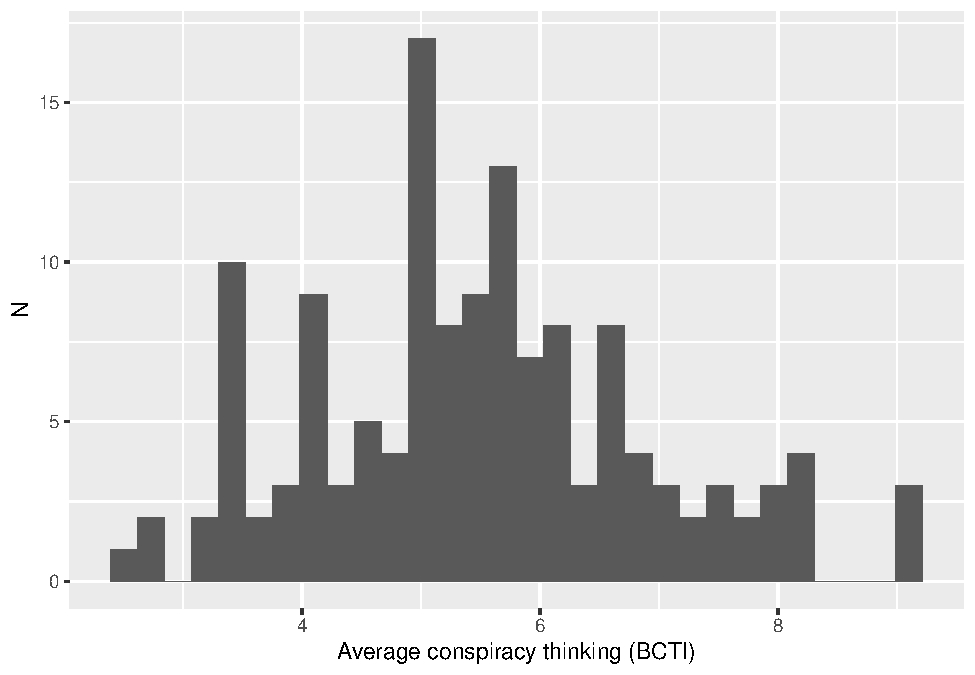
\includegraphics{output/figures/exp3-conspiracy-distribution.pdf}
\caption{\label{fig:exp3-conspiracy-distribution}Distribution of conspiracy thinking.}
\end{figure}

\subsubsection{By-item variation}\label{by-item-variation-2}



\begin{figure}
\centering
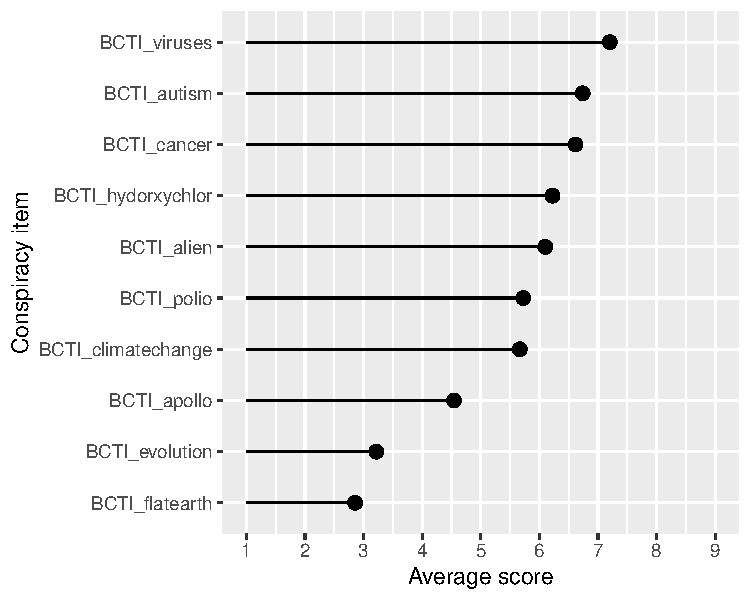
\includegraphics{output/figures/exp3-conspiracy-items.pdf}
\caption{\label{fig:exp3-conspiracy-items}Distribution of conspiracy thinking by item.}
\end{figure}

\subsection{Reasons for consensus rejection}\label{reasons-for-consensus-rejection-1}

\subsubsection{All raw answers}\label{all-raw-answers-1}

\begin{longtable}[t]{>{}r>{}l>{\raggedright\arraybackslash}p{30em}}
\caption{\label{tab:exp3-reasons-rejection}Reasons for consensus rejection}\\
\toprule
id & question & answer\\
\midrule
5 & lasers & It is what I believed I was taught\\
12 & antibiotics & I do not know\\
20 & water & I think I got it confused in my head. I was thinking 2 oxygen and 1 hydrogen.\\
25 & electrons & I made a mistake.\\
26 & antibiotics & I have always experienced receiving antibiotic for viral infections. So i do not agree that antibiotic does not kill viruses.\\
\addlinespace
32 & antibiotics & Because I realized that my thinking was not correct.\\
32 & orbit & After thinking about it, I realized  that it does take a year for the sun to go around the earth.\\
38 & continents & The earth is not millions of years old.\\
38 & orbit & The earth is flat and stationary.\\
43 & water & I got it confused. Its true. One oxygen and  2 hydrogen is what i learned in school.\\
\addlinespace
46 & sex & Yes.  Its normal to think that, however, not always.\\
53 & continents & The Earth was created aged by God and has not been around for millions of years. I do not believe in evolution but rather creation based on the Word of God.\\
61 & continents & I do not believe that the universe is millions of years old\\
62 & continents & I do not believe the theory that the earth is that old.\\
65 & electrons & Because I would like to see more research on this matter.\\
\addlinespace
65 & antibiotics & Because I would like to see more research on this matter.\\
65 & continents & Because I would like to see more research on this matter.\\
65 & diamonds & Because I would like to see more research on this matter.\\
65 & water & Because I would like to see more research on this matter.\\
72 & lasers & That’s the truth\\
\addlinespace
72 & salt & I wasn’t sure\\
83 & continents & The Earth has only been around for 6-7 thousand years. As far as I know however, the Continents have been moving.\\
83 & water & thought it was "2 parts oxide, one hydrogen." I was of course wrong. I also miss clicked the wrong answer for how long it takes the Earth the revolve around the sun... I think.\\
87 & electrons & I believe atoms are the smallest particles.\\
87 & continents & On second thought, I agree.\\
\addlinespace
87 & diamonds & On second thought, I believe I agree.\\
87 & water & This does not fit according to my recollection.\\
92 & salt & I meant to agree, I did not know the answer.\\
96 & electrons & I don't think electrons are smaller, just because that is what we were taught in science\\
96 & continents & This is something we are taught academically in science, it may not be true\\
\addlinespace
98 & antibiotics & I think there are two different kinds of antibiotics. One type kills bacteria infections and the other type kills viral infections\\
99 & continents & I don't have a reason to believe Earth has been here for millions of years, so I don't agree with the consensus. Of course, I know I could be wrong.\\
102 & continents & This information is based in evolution which is a theory.\\
109 & continents & I partially agree that continents have moved due to plate tectonics. But I don't believe the Earth is as old as it mentions in the explanation, and is much younger. I also disagree with scientific consensus and there is really no such thing. Because with science, when you base things on evidence and then find new evidence, you have to change your theory. So there is really no such thing as consensus, there is data, facts and theories.\\
112 & antibiotics & No\\
\addlinespace
112 & speed & No\\
112 & salt & No\\
117 & antibiotics & Not really. I thought they killed virus' but maybe I am wrong. heh.\\
117 & sex & I thought both male and female decided the fate of the babies gender.\\
122 & antibiotics & antibotics only kill bacteria\\
\addlinespace
122 & lasers & I thought they light was a lot faster than sound waves\\
122 & salt & not sure\\
129 & continents & YES, I believe in a young earth.  I do not accept the tax supported theory of evolution.\\
130 & antibiotics & I was confused.\\
132 & continents & Continental drift is an unproven theory. I have seen no actual evidence for it. Flooding and receding of waters are more likely the cause of coastline changes throughout history.\\
\addlinespace
132 & orbit & There is no scientific evidence that the earth moves at all except for earthquakes. The sun is clearly moving around the earth in a daily circular pattern. The sun is much smaller and closer than we have been taught.\\
142 & salt & I thought it was made up of that.\\
143 & lasers & Lasers operate based on the principles of stimulated emission of electromagnetic radiation, typically light.\\
146 & antibiotics & Different knowledge and experience.\\
146 & sex & A mothers choice not the fathers choice because of religious beliefs.\\
\addlinespace
146 & diamonds & Gained through knowledge and skills.\\
150 & speed & To be honest, I did actually hear the concept that like travels fashion and sound so I’m not sure why I picked that answer.\\
151 & lasers & I accidentally clicked the other answer I'm not going to lie. As soon as I clicked it on accident I was like "Sh*t". I meant to choose the other answer on this one, I'm sorry.\\
151 & salt & I misunderstood this question. This one confused me the most even though it's right in front of me. Sorry.\\
155 & salt & error\\
\addlinespace
158 & lasers & No I did not know this question.\\
158 & salt & I knew this one and just blanked on the answer.\\
159 & sex & I thought I read it said in most cases women transmit an X chromosome, but now I'm not sure.\\
161 & antibiotics & I thought antibiotics kills every bit of poison.\\
166 & electrons & I'm not sure, I dont' understand it\\
\addlinespace
166 & water & I'm not sure, I dont' understand it\\
171 & diamonds & It just doesn't sit well with me.\\
172 & sex & I was wrong. I agree with scientific consensus.\\
173 & orbit & Yes the scientist now more than I do\\
178 & electrons & I was incorrect on this.\\
\addlinespace
191 & antibiotics & I could be wrong, but I thought they killed viruses as well.\\
191 & continents & I do not believe without a doubt the earth has been around for millions of years.\\
196 & sex & Answered incorrectly in error.  I agree with the scientific consensus.\\
197 & antibiotics & I’ve taken antibiotics numerous of times and although my sickness is usually cured, I always get a yeast infection as result. This always happens since the antibiotics kill the good and bad bacteria in the body.\\
197 & sex & I believe that God decides whether parents will be blessed with a boy or girl. It had nothing to do with genetics.\\
\addlinespace
197 & diamonds & This just doesn’t seem correct even after viewing the article from the university. I can’t explain why but I can’t justify it.\\
198 & diamonds & I just never heard of diamonds being made of carbon and it makes zero sense to me while thinking about it.\\
200 & continents & The earth is not old but young. Not billions or millions but thanks of years.\\
200 & orbit & One day because the sun is not taking a year to light up other parts of the earth.\\
\bottomrule
\end{longtable}

\subsection{Why do people accept the scientific consensus:}\label{why-do-people-accept-the-scientific-consensus}

\subsubsection{Participants who answered ``other''}\label{participants-who-answered-other}

\begin{longtable}[t]{>{}r>{\raggedright\arraybackslash}p{30em}}
\caption{\label{tab:exp3-other-reasons-acceptance}Reasons for consensus rejection}\\
\toprule
id & other\_reason\_agreement\\
\midrule
24 & some stuff I already knew, other stuff I don't care about like atoms and molecules\\
37 & I mostly agreed based on my personal knowledge.\\
62 & I have never seen compelling evidence to disprove the consensus.\\
89 & Because it is true.\\
101 & I can't say that I trust scientists on many things, but on most in this survey. However, while I believe the continents have moved around, I don't believe the earth is millions of years old, as I'm a Christian. Though God never notes exactly how old the earth is, so it could be millions of years old.\\
\addlinespace
102 & Agreed due to vague knowledge about the subject.\\
166 & I'm not sure, you cant trust any party\\
172 & Because i recall previously being taught that\\
182 & I agree because the explaination makes sense\\
188 & I don't trust scientists, but those are the current established 'facts'. Which, on the mundane side of things, are likely true.\\
\addlinespace
189 & I take nothing that anyone tells me at face value. Lots of studying and verifying accuracy of the things that I was taught my entire life.\\
195 & I mostly agree with the consensus because I don't have the equipment to independently test it myself and I also know scientists have proven those who don't have the so called equipment to know what they know. We can only observe what we observe at the moment, but there's more to what the scientists are observing and theorizing.\\
\bottomrule
\end{longtable}

\subsection{How did participants independently verifiy?}\label{how-did-participants-independently-verifiy}

\subsubsection{Participants who answered ``other''}\label{participants-who-answered-other-1}

\begin{longtable}[t]{>{}r>{\raggedright\arraybackslash}p{30em}}
\caption{\label{tab:exp3-independent-verification}Reasons for consensus rejection}\\
\toprule
id & reason\_followup\\
\midrule
5 & By trying to remember\\
10 & Curiosity and the internet\\
12 & Guessed\\
14 & I double-checked the information on Google by looking up various websites, I did go with my initial gut instincts in most cases however if it was wrong upon verifying it then I would change my answer\\
18 & Prior knowledge from a formal education\\
\addlinespace
19 & I can check several different sources on the internet and see if they have the same verifiable information.\\
21 & I use intuition.  I use common sense.\\
22 & I have read it before, and did some experiments in chemistry class.  I look for scientific consensus on everything.  On these long established principles, I could have selected both answers.  I believe sometimes scientists are bribed or exhibit bias depending on who is funding them and what answers the funding entity wants. COVID treatments were a big example of that.  Hospitals were paid to execute certain protocols and disallow others.\\
27 & Most of the questions, the consensus answer was the same as my answer. For the one or two questions where it was not, I looked at who their sources were for the answers, and decided whether I believed those sources and how unsure I was about my answer and made my decision from there.\\
31 & Through exposure to scientific experiments and research that prove the claims valid and can be repeated with the same results occurring.\\
\addlinespace
36 & There is evidence and a good amount of understand about these issues. There isn't as much understanding when it comes to things like vaccines.\\
38 & Through many sources, including my own common sense and a lifetime of research into these matters.\\
39 & I used the information that I have learned in school and in the past.\\
40 & Most things I knew already as some were common knowledge\\
41 & My gut instinct.\\
\addlinespace
42 & Most was knowledge I already knew, however if I were to find out or look up info, I would simply consult the internet\\
43 & I thought about what i was told in school.\\
44 & I checked reliable sources, and I knew most of them from learning this information in science class.\\
48 & some things are obvious and don't need verification\\
49 & Research on my own as opposed to jist blindly following what the media is told to tell me.\\
\addlinespace
56 & extensive research\\
58 & I verified it with what then knowledge I know\\
67 & I remember some of the stuff from school.\\
68 & I clicked on two out of three of the links for most statements that I was unsure about.\\
71 & I have a lot of people who do deep research that verified the info.\\
\addlinespace
77 & Just various amounts of research online. There have been times where simple questions were simply ignored or answered in a perplexing manner. Those types of answers always raise a flag.\\
81 & By  the knowledge I already had.\\
82 & Some of these questions I remember from high school. And I learned this in science. Therefore I do remember alot of these questions.\\
88 & I don't know\\
97 & Either I already knew the information or after reading the information I can to my conclusion\\
\addlinespace
98 & My wife has taken two different kinds of antibiotics, one for viral infections and one for bacterial infections\\
100 & I independently verified the information by doing a lot of research and comparing studies.\\
103 & I do my own research.\\
114 & I guess I haven't independently verified the information.\\
116 & wikipedia articles and google searches\\
\addlinespace
120 & The questions I got wrong were facts that I had simply forgotten. Once made aware of the correct answer, I remembered that it was in fact the correct answer.\\
122 & heard of it before\\
123 & I used the links provided and then googled the question if I was unsure\\
126 & It is an obvious pattern whenever these events happen that there is a coverup, you just have to research the track record\\
129 & I'm unsure of which question, you asked several.  it's a bit confusing. the vaccine question has been verified by personal treatment and independent studies that were banned on social platforms\\
\addlinespace
131 & I used the information and links given to verify it.\\
132 & I have been studying this information for many years. Real science is not consensus alone. Peer review is rigged and fraudulent. We are not being given the truth about many things and most "scientists" don't even know that they are wrong and refuse to reinvestigate the topics.\\
136 & Have an educational background in anthropology and took a lot of science courses. I trust scientists generally but not always the way the findings are relayed.\\
137 & My own research, we were lied to in school\\
144 & By looking through multiple sources on a given topic.\\
\addlinespace
152 & A lot of this I have already learned, but I can't personally verify it bc I can't run the tests.\\
154 & I have done several science experiments to prove a lot of these ideas.\\
156 & looking it up online from at least 2-3 sources\\
159 & Instead of taking what the mainstream talking point is and immediately accepting it, I like to do further research myself.\\
161 & I already knew of the information presented to me for years.\\
\addlinespace
163 & I googled it and read information from various sources.\\
164 & Many of these tidbits of information are taught as introduction to different subjects. I have either studied this or have used Google  Academic to verify.\\
178 & Some of the questions I've done my own research on, others I can see with my own eyes.\\
185 & most of the questions i already knew the answer to because i researched it a long time ago\\
186 & The information presented is basic knowledge we learn throughout ours lives. Light travels faster than sound. The fathers genes decide whether ba baby will be male or female. Diamonds are formed from carbon. Calcium carbonate is not sodium chloride. It takes the earth 365.2ish to orbit our sun. Yes, water is 2 hydrogen, 1 oxygen. And and electron is much smaller than an atom. All things we learn in school. Oh and lasers use light waves not sound waves.\\
\addlinespace
187 & For light traveling faster then sound it's obviously verifiable because you see lightning before you hear thunder, lasers are visible so obviously they are made of light not sound, the definition of water is H2O so if something isn't H2O then it isn't water.  The vast majority of the questions were extremely common sense if you think about them for any amount of time.\\
191 & I either realized I was wrong or it sounded logical in my mind.\\
200 & The Bible.\\
\bottomrule
\end{longtable}


\end{document}
